%
% Configuratie
%

% Preambule met standaardinstellingen
\documentclass[a4paper,oneside]{report}

% Noot: zorg ervoor dat Nederlandse woordsplitsing geactiveerd is.
\usepackage[english,dutch]{babel}

% Noot: je kan het graphicxpakket een optie dvips of pdftex doorgeven
% in dat geval moet je ze ook aan iiiscriptie doorgeven, dus bijvoorbeeld
% \usepackage[dvips]{graphicx}
% \usepackage[dvips]{iiiscriptie}
\usepackage{graphicx}
\usepackage{iiiscriptie}

% Nuttig pakket voor URL's
\usepackage{url}

% Genereer een index
% gebruik \index{tekst} om een index toe te voegen
\usepackage{makeidx}
\makeindex

% Extra functies
% Verkleinde margin entry
\setlength{\marginparwidth}{1.2in}
\let\oldmarginpar\marginpar
\renewcommand\marginpar[1] {\-\oldmarginpar[\raggedleft\footnotesize #1]%
{\raggedright\footnotesize #1}}

% Een TODO-entry
\newcommand{\todo}[1] {
	\addcontentsline{tdo}{todo}{\protect{#1}}
	\marginpar{#1}
}

% Een lijst van TODO-entries
\makeatletter
\newcommand \listoftodos {
	\section*{Todo list} \@starttoc{tdo}
}
\newcommand\l@todo[2] {
	\par\noindent \textit{#2}, \parbox{10cm}{#1}\par
} \makeatother

% Float defini\"eren voor codefragmenten
\usepackage{float}
\floatstyle{ruled}
\newfloat{code}{thp}{lop}
\floatname{code}{Codefragment}

% Hyperlink maken en URL in footnote tonen
\usepackage{hyperref}
\newcommand{\makeurl}[2]{\href{#2}{#1} \footnote{#2}}

% Functiedefinitie voor protocolstudie
\newcommand{\function}[5] {
	\subsubsection*{#1}
	\begin{tabular}{|r p{11cm}|}
	\hline
	\textsc{Gebruik} |		& #2 \\
	\textsc{Parameters} |		& #3 \\
	\textsc{Output} |		& #4 \\
	\textsc{Autorisatie} |		& #5 \\
	\hline
	\end{tabular}
}

% Functiedefinities voor logboek handling
\usepackage{ifthen}
\newcommand{\lbdate}{}
\newcommand{\lbsetdate}[1]{
  \gdef\lbdate{#1}
}
\newcommand{\lbentry}[5] {
	\ifthenelse{\equal{\lbdate}{#1}}
	{
	}
	{
		\ifthenelse{\equal{\lbdate}{}}{}{
			& & & \\ \hline % TODO: workaround, zou niet nodig moeten zijn
			\end{tabular}
		}
		\subsection*{#1}
		\begin{tabular}{|r r r p{10cm}|}
		\hline
		\textsc{Begin} & \textsc{Einde} & \textsc{Duur} & \textsc{Beschrijving} \\
		\hline
	}
	\lbsetdate{#1}
	#2 & #3 & #4 & #5 \\
}
\newcommand{\lbstop}[1] {
	& & & \\ \hline % TODO: consistentie fix, zie hierboven
	\end{tabular}
	\lbsetdate{}
	
	\subsection*{Sommatie}
	\textbf{Totale aantal werkuren}: #1.
}

% Compacte enumeraties
\newenvironment{enumerate_compact}{
\begin{enumerate}
  \setlength{\itemsep}{1pt}
  \setlength{\parskip}{0pt}
  \setlength{\parsep}{0pt}
}{\end{enumerate}}
\newenvironment{itemize_compact}{
\begin{itemize}
  \setlength{\itemsep}{1pt}
  \setlength{\parskip}{0pt}
  \setlength{\parsep}{0pt}
}{\end{itemize}}

% Compacte environment voor use-cass
\newenvironment{compact}{\setlength{\parskip}{0pt}}{}

%stijlen voor listings
%
\lstdefinestyle{SQL}{
  breaklines=true,
  language=SQL,
  basicstyle=\normalsize,
  keywordstyle=\ttfamily\color{OliveGreen},
  identifierstyle=\ttfamily\color{CadetBlue}\bfseries,
  commentstyle=\color{Brown},
  stringstyle=\ttfamily,
  showstringspaces=true
}


\definecolor{myid}{rgb}{0.1,0.1,0.1}
\lstdefinestyle{Java}{
language=java,
basicstyle=\normalsize,
numbers=left,stepnumber=1,numberstyle=\small\ttfamily,
numbersep=5pt,frame=tlbr,extendedchars=true,
commentstyle=\color{OliveGreen}\ttfamily,
%% stringstyle=\color{red}\ttfamily,
stringstyle=\ttfamily\color{Magenta},
keywordstyle=\ttfamily\color{Violet}\bfseries,
ndkeywordstyle=\ttfamily\color{Yellow}\bfseries,
identifierstyle=\ttfamily\color{myid},
% sensitive=false,
}



%
% Titelpagina
%

% Invullen velden
\departement{Departement Toegepaste Ingenieurswetenschappen}
\deptadres{Schoonmeersstraat 52 - 9000 Gent}
\studiejaar{3e Bachelor Informatica}
\soortrapport{
Analyse voor het vakoverschrijdend project Informatica
}
\title{Verslag 'StockPlay'}
\author{
Tim BESARD\\
Dieter DEFORCE\\
Laurens VAN ACKER\\
Thijs WALCARIUS
}

% Pagina maken
\begin{document}
\maketitle
\pagenumbering{roman}
\tableofcontents
\pagenumbering{arabic}


%
% Inhoud
%

% Inleiding
\chapter*{Inleiding}
StockPlay is een spel waarmee beleggen op de beurs wordt gesimuleerd. De deelnemers kunnen aandelen, opties, trackers, fondsen, enz. verhandelen (later "effecten" genoemd). De bedoeling van het spel is om een zo goed mogelijke prestatie neer te zetten: zowel de continue prestaties, alsook het rendement op het einde van het spel zijn belangrijk.

% Analyse
\part{Analyse}
%
% Definitiestudie
%

\section{Definitiestudie}

Voorafgaand aan de start van het spel is er een inschrijvingsperiode. (Uitbreiding: Spelers kunnen zich registeren met behulp van hun eID.) Spelers die zich registeren voor de start van het spel verkrijgen 100.000 euro virtuele cash.

Het spel start op een vastgesteld moment: op 1 maart 2010 om 8u 's morgens, Central European Time. Gebruikers die na de start van het spel registreren krijgen een ander startbudget. Maximaal verkrijgen de spelers een startbudget van 100.000 euro. Is de re\"ele beurs sinds de start van het spel negatief ge\"evolueerd, dan wordt het startbudget ook in verhouding evenveel verlaagd.

Van zodra gebruikers geregistreerd zijn, hebben de gebruikers toegang tot hun portfolio en kunnen daar effecten aan worden toegevoegd.

De gebruiker kan effecten aankopen en verkopen van onderstaande types:
\begin{itemize_compact}
	\item{aandelen op de Continumarkt van Brussel}
	\item{aandelen op de Eurolist van Parijs}
	\item{aandelen op de Lokaal van Amsterdam}
	\item{trackers op Euronext Amsterdam}
\end{itemize_compact}

Tijdens het verloop van het spel worden er op gezette tijden (per dag, per week en per maand) klassementen opgemaakt met daarin het relatief rendement dat de spelers konden neerzetten. Op basis van deze tussenklassementen worden er ook punten toegekend, waarmee ook een apart puntenklassement wordt opgemaakt. Dit puntenklassement geeft een eerlijkere kijk op de prestaties van de speler, en zorgt ervoor dat niet enkel het uiteindelijke rendement tussen de start- en einddatum van belang is, maar ook de continue goede prestaties tijdens de duur van het spel.

Het spel eindigt op 31 mei 2010, waarna een eindklassement wordt opgemaakt. De koersen op de website worden niet meer geüpdatet, en er kunnen ook geen transacties meer gedaan worden. Gebruikers kunnen wel nog steeds authenticeren op de website om statistieken van hun spelverloop te raadplegen.


\subsection{Website}

\begin{figure}[h!]
	\centering
		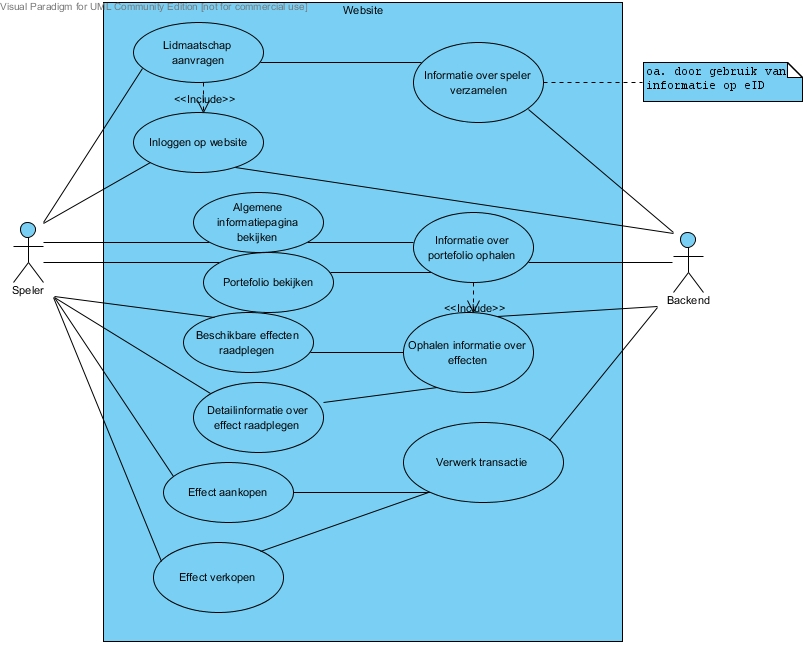
\includegraphics[width=0.5\textwidth]{images/analyse/ucd_website}
	\caption{Use-case diagram van de website.}
\end{figure}

\paragraph{Lidmaatschap aanvragen}
\begin{compact}
\subparagraph{Beschrijving}Een persoon kan zich inschrijven voor een lidmaatschap. Dit lidmaatschap is een vereiste om de interactieve delen van de website te kunnen beleven. Deze procedure bestaat uit een aantal velden die naar waarheid in te vullen zijn en een aantal velden waar men een waarde voor kan kiezen.
\subparagraph{Primaire actoren}Een persoon die de interactieve delen van de website wil gebruiken
\subparagraph{Doel}De speler verkrijgt een lidmaatschap. Via dit lidmaatschap kunnen we een persoon (een speler) koppelen aan zijn portfolio.
\subparagraph{Precondities}De speler bezitte een geldig email adres, een eID lezer en hij was nog niet in bezit van een lidmaatschap (een persoon bezit een lidmaatschap als hij de combinatie gebruikersnaam en wachtwoord kent of over een eID bezit waar een lidmaatschap aan gekoppeld is). \small{Lidmaatschap aanvragen is pas mogelijk vanaf 1 maart 2010, 8u, Central European Time.}
\subparagraph{Postcondities}In de database zit een nieuw record waarmee we de speler kunnen authenticeren en waaraan zijn instellingen en portfolio gekoppeld worden.
\subparagraph{Triggers}Een persoon zit op de inleidende website en kiest daar voor de optie ``Registreren''.
\subparagraph{Notities}De velden die de gebruiker op de afzonderlijke registratie pagina dient in te vullen zijn terug te vinden in het database schema van de gebruikers. Alle velden zijn verplicht.
\subparagraph{Business rules}Het registreren (en dus onrechtstreeks het spelen van het beursspel) moet aangemoedigd worden vanuit de gastsite.
\subparagraph{Prioriteit}Gemiddeld
\subparagraph{Complexiteit}Laag
\subparagraph{Successcenario}
\begin{enumerate_compact}
 \item Speler bezoekt de website
 \item Speler maakt de keuze dat hij mee wil spelen
 \item Speler geeft aan te willen registreren
 \item Speler vult alle vereiste velden in
 \item Speler vult eventueel enkele optionele velden in
 \item Speler bevestig zijn registratie
 \item \label{def:lidmaatschap:bevestiging} Speler krijgt een bevestiging van zijn registratie
\end{enumerate_compact}
\subparagraph{Alternatieve scenario's}
Alternatief voor \ref{def:lidmaatschap:bevestiging}:
\begin{itemize_compact}
 \item Speler is een vereist veld vergeten en krijgt de mogelijkheid om dit aan te passen
 \item Speler heeft een ongeschikte of foutieve invoer gedaan voor een veld en krijgt de mogelijkheid om dit aan te passen
\end{itemize_compact}
\end{compact}
 
\paragraph{Het bekijken van de gastsite}
\begin{compact}
\subparagraph{Beschrijving}De website zal uit drie delen bestaan. Een deel bestaat uit een of meerdere pagina's. Een deel zal enkel zichtbaar zijn voor niet geauthenticeerde gebruikers of bezoekers zonder lidmaatschap. Een ander deel zal zichtbaar zijn voor zowel niet geauthenticeerde bezoekers als geauthenticeerde bezoekers. Geauthenticeerde bezoekers hebben dan ook nog toegang tot een enkel voor hen zichtbare derde deel. Het is in dat deel dat de interactieve site zich bevindt.
\subparagraph{Primaire actoren} Bezoekers zonder lidmaatschap die er wel een willen aanvragen, bezoekers zonder lidmaatschap die enkel op zoek zijn naar informatie over het spel en bezoekers met lidmaatschap die zich willen authenticeren voor toegang tot het voor hen zichtbare deel.
\subparagraph{Doel} Bezoekers snel laten inloggen, bezoekers informeren over het spel, bezoekers doorheen de registratieprocedure leiden.
\subparagraph{Precondities} De gastsite heeft dezelfde precondities als de overige delen van de website. De surfer was voorzien van een breedband internetverbinding, een desktop of draagbare computer met daarop een gangbaar en recent besturingssysteem en bijhorende standaard compatibele internetbrowser.
\subparagraph{Postcondities} De gebruiker was ingelogd, geregistreerd of was voldoende ge\"informeerd over het spel.
\subparagraph{Triggers} De surfer bezoekt de website door het ingeven van het webadres, het aanklikken van een favoriet in zijn internetbrowser of na het klikken op een webverwijzing op een andere internetwebsite.
\subparagraph{Notities} Het gastgedeelte zal op elke pagina een module bevatten waarmee bezoekers met lidmaatschap zich snel kunnen authenticeren.\small{Om de surfer te informeren over het spel zullen verschillende pagina's voorzien worden. Op die pagina's zijn visuele hulpmiddelen voorzien zoals afbeeldingen waarop te zien is hoe bepaalde spelprocedures verlopen en eventueel ook ondersteunde filmen.}
\subparagraph{Business rules}Het is op dit gedeelte van de site dat de surfer en potenti\"ele speler overtuigd moet worden om actief mee te spelen.
\subparagraph{Prioriteit}Laag
\subparagraph{Complexiteit}Laag
\subparagraph{Successcenario}
\begin{enumerate_compact}
 \item Speler bezoekt de website
 \item Speler navigeert naar de juiste pagina
 \item Speler is voldoende ge\"informeerd
\end{enumerate_compact}
\end{compact}

\todo{De beschrijving van deze use case is gewoon een kopie van de vorige?? -Dieter}
\paragraph{Inloggen}
\begin{compact}
\subparagraph{Beschrijving} De website zal uit drie delen bestaan. Een deel bestaat uit een of meerdere pagina's. Een deel zal enkel zichtbaar zijn voor niet geauthenticeerde gebruikers of bezoekers zonder lidmaatschap. Een ander deel zal zichtbaar zijn voor zowel niet geauthenticeerde bezoekers als geauthenticeerde bezoekers. Geauthenticeerde bezoekers hebben dan ook nog toegang tot een enkel voor hen zichtbare derde deel. Het is in dat deel dat de interactieve site zich bevindt. Dat deel is enkel toegankelijk voor geauthenticeerde bezoekers.
\subparagraph{Actoren} Bezoekers met lidmaatschap die toegang willen tot het interactieve deel van de website.
\subparagraph{Doel} Een bezoeker koppelen aan zijn lidmaatschap en dus onrechtstreeks aan zijn portfolio, puntentotaal en instellingen.
\subparagraph{Precondities} De bezoeker bezit reeds een lidmaatschap en beschikt over voldoende informatie en hulpmiddelen om aan te kunnen tonen dat dit lidmaatschap van hem of haar is.
\subparagraph{Postcondities} De gebruiker is geauthenticeerd.
\subparagraph{Triggers} De gebruiker vult zijn gebruikersnaam en wachtwoord in of verbind zijn eID met de applicatie. Dit gebeurt vanaf de gastpagina.
\subparagraph{Notities} Het kan zijn dat de gebruiker niet moet inloggen omdat dit reeds voorheen gebeurd is en een bepaald mechanisme met een cookie de authenticatie reeds verzocht heeft. Dit laatste gebeurt dan onzichtbaar voor de gebruiker.
\subparagraph{Prioriteit}Hoog
\subparagraph{Complexiteit}Hoog
\subparagraph{Successcenario}
\begin{enumerate_compact}
 \item Speler bezoekt de website
 \item Speler geeft voldoende gegevens waarmee hij zich kan authenticeren
 \item \label{def:inloggen:bevestiging} Speler krijgt een bevestiging en wordt doorgestuurd naar het interactieve deel van de website
\end{enumerate_compact}
\subparagraph{Alternatieve scenario's}
Alternatief voor \ref{def:inloggen:bevestiging}:
\begin{enumerate_compact}
 \item Speler heeft een ongeschikte of foutieve invoer gedaan voor een veld en krijgt de mogelijkheid om dit aan te passen
\end{enumerate_compact}
\end{compact}

\paragraph{De gebruiker bekijkt zijn eigen Portfolio}
\begin{compact}
\subparagraph{Beschrijving} De gebruiker ziet een webpagina met daarop de effecten die deze momenteel in bezit heeft, de historische aankoopprijs per stuk, de historische aankoopprijs in totaal, de huidige koers, het rendement en het verschil op de waarde sinds de aankoop van het effect.
\subparagraph{Actoren} De speler bekijkt het portfolio. De huidige waarde hangt af van de re\"ele beursevolutie (de scrapers volgen deze evolutie).
\subparagraph{Doel} De gebruiker ziet zijn portfolio en de gegevens die interessant zijn om erbij te zien.
\subparagraph{Precondities} De gebruiker is ingelogd.
\subparagraph{Triggers} De gebruiker kiest in het linkermenu de optie ``Portfolio''.
\subparagraph{Prioriteit}Hoog
\subparagraph{Complexiteit}Laag
\subparagraph{Successcenario}
\begin{enumerate_compact}
 \item De gebruiker geeft aan zijn portfolio te willen bekijken
 \item De gebruiker definieert een filtering of een combinatie van filters
 \item Een overzicht van de speler zijn huidige portfolio wordt getoond
\end{enumerate_compact}
\end{compact}

\todo{In deze use case staan al die verschillende orders beschreven. Maar die staan al uitgewerkt in ``Module geavanceerde orders''! Het lijkt me best om hier gewoon een opsomming te geven van de mogelijkheden en te refereren naar dat ander hoofdstuk.}
\paragraph{Effecten aankopen}
\begin{compact}

\subparagraph{Overzicht}Een gebruiker kan zijn portfolio invullen of aanvullen door effecten bij te kopen. De speler kan effecten bijkopen van een effect die hij/zei reeds bezit of een nieuwe reeks aankopen. Een effect kan nooit rechtstreeks aangekocht worden, dit gebeurt met een tussenstap. Deze tussenstap noemen we het plaatsen van een order. Een order bestaat er in twee types; een aankooporder of een verkooporder. Een order heeft een voorwaarde, type, aantal, eigenaar en effect. Orders worden periodiek (elke minuut) bekeken. Als aan de voorwaarde voldaan wordt, dan wordt het order omgezet in een effectieve aankoop of verkoop. Dan pas worden de effecten toegevoegd of verwijderd van het spelers portfolio. Het kan dus zijn dat een geplaatst order pas in de verre toekomst uitgevoerd wordt of in zijn geheel niet uitgevoerd wordt. De voorwaarden die op een order ingezet kunnen worden houden we in een eerste fase beperkt. Maar deze kunnen later aangevuld worden met geavanceerde orders, zoals ook te zien is bij de huidige gespecialiseerde brokers. We beginnen met drie typen van orders:

\begin{itemize_compact}
 \item Voer onmiddellijk uit, ongeacht de huidige koers.
 \item Koerslimiet: Voer een aankoop order uit als de prijs lager is dan de ingestelde limietwaarde
 \item Koerslimiet: Voer een verkoop order uit als de prijs hoger is dan de ingestelde limietwaarde
\end{itemize_compact}

Mogelijke geavanceerde orders die we in een verdere fase zouden kunnen invoeren zijn de volgende:
\begin{itemize}
	\item \emph{Trailling-stop}: Bij een verkoop order wordt de trigger waarde ingesteld op een vast aantal beurspunten onder de hoogste koers. Als de hoogste koers dus verhoogd in waarde, dan verhoogd ook de trigger waarde evenveel punten. Deze tactiek gebruikt de speler als die verwacht dat de waarde van het effect nog wel een tijdje zal toenemen, maar hij toch zijn winst wil veiligstellen. Hetzelfde kan ook ingesteld worden bij een aankooporder. Als de speler namelijk verwacht dat de waarde van een effect nog een tijdje zal blijven dalen, en de speler laag wil inkopen.
  \item \emph{Bracket-limiet}: De speler kan met dit type order de maximale fluctuaties van zijn effect beperken. Hij stelt twee waardes in waar het order omgezet zal worden in een effectieve handeling. Dit is een waarde boven de huidige koers en een waarde onder de huidige koers. Zo beperkt de speler dus zijn maximaal verlies, maar ook zijn maximale winst. De waardes tussen de hoogste en laagste limietwaarde is de bandbreedte waar het effect kan tussen schommelen terwijl het in de portefeuille blijft van de speler.
  \item \emph{Stop loss order}: Een order wordt omgezet in een effectieve handeling ongeacht de limietwaarde. Het order wordt hierdoor sneller uitgevoerd, maar er is geen minimumprijs (maximumprijs) gegarandeerd.
\end{itemize}
\subparagraph{Prioriteit}Laag
\subparagraph{Complexiteit}Laag
\subparagraph{Successcenario}
\begin{enumerate_compact}
 \item Speler geeft vanuit een overzichtspagina of detailpagina aan dat hij een order wil plaatsen op een effect
 \item Speler geeft de order specificaties op (aantal effecten, type, limieten, )
 \item Speler bevestigd zijn order
 \item \label{def:aankopen:bevestiging} Speler krijgt een bevestiging van zijn order
\end{enumerate_compact}
\subparagraph{Alternatieve scenario's}
Alternatief voor \ref{def:aankopen:bevestiging}:
\begin{enumerate_compact}
 \item Speler heeft een ongeschikte of foutieve invoer gedaan voor een veld en krijgt de mogelijkheid om dit aan te passen
\end{enumerate_compact}
\end{compact}

\paragraph{Effecten verkopen}
\begin{compact}
Een effect verkopen verloopt op dezelfde manier als een effect aankopen. Er wordt ook een order aangemaakt voor een aantal effecten. Resulteert de voorwaarde van het order positief, dan worden zoveel effecten verkocht. Als een gebruiker geen effecten meer overhoudt van een bepaald symbool, dan wordt dit uit het portfolio gehaald.
\subparagraph{Actoren} De speler plaatst een order
\subparagraph{Doel} Een order plaatsen welke tot doel heeft omgezet te worden in een effectief order. Dit wordt bepaald door de voorwaarde die ge\"evalueerd wordt ten op zichte van de huidige beursevolutie. Het onrechtstreekse doel is het uitbreiden van het virtueel portfolio van de speler.
\subparagraph{Precondities} De gebruiker zijn cash positie moet voldoen om het order te plaatsen en uit te voeren.
\subparagraph{Postcondities} Een order is geplaatst en kan later uitgevoerd worden, mislukken of verlopen.
\subparagraph{Triggers} De aankooppagina wordt getoond door het activeren van een optie op een effectenpagina.
\subparagraph{Prioriteit}Laag
\subparagraph{Complexiteit}Laag
\subparagraph{Successcenario}
\begin{enumerate_compact}
 \item Speler geeft vanuit een overzichtspagina of detailpagina aan dat hij een order wil plaatsen op een effect
 \item Speler geeft de order specificaties op (aantal effecten, limieten, )
 \item Speler bevestigd zijn order
 \item \label{def:verkopen:bevestiging} Speler krijgt een bevestiging van zijn order
\end{enumerate_compact}
\subparagraph{Alternatieve scenario's}
Alternatief voor \ref{def:verkopen:bevestiging}:
\begin{enumerate_compact}
 \item Speler heeft een ongeschikte of foutieve invoer gedaan voor een veld en krijgt de mogelijkheid om dit aan te passen
\end{enumerate_compact}
\end{compact}

\paragraph{Overzicht opvragen van de effecten die je in het spel actief kan verhandelen}
\begin{compact}
\subparagraph{Beschrijving} Een effect op de beurs kan ofwel opgenomen worden door onze scrapers of buiten bereik liggen van onze scrapers.
Als deze binnen het bereik van een of meerdere scrapers valt, dan worden er gegevens van bijgehouden in onze dataopslag. Een effect kan dan nog onderverdeeld worden onder effecten die onzichtbaar zijn op de site, effecten die geschorst zijn en dus niet actief verhandeld kunnen worden en actief te verhandelen effecten. Bij het overzicht worden de gescrapete actieve of geschorste effecten getoond. Hierop kunnen dan filters geplaatst worden om de lijst in te korten.
\subparagraph{Doel} Een effect kunnen vinden waarvan je de detailpagina wil bekijken. Met het onrechtstreekse doel op het geschikte effect een order te plaatsen. Een detail pagina vind je door in het overzicht een aandeel aan te klikken.
\subparagraph{Postcondities} De speler ziet een pagina met daarin een lijst van effecten die voldoen aan zijn ingestelde of geselecteerde filter
\subparagraph{Triggers} Via het menu vraagt de speler de overzichtspagina op
\subparagraph{Notities} Er kan een combinatie van volgende filters ingesteld worden op de site:

\begin{itemize_compact}
	\item Type
	\item Beurs
	\item Index
	\item Deelstring van de naam
	\item Effecten met een vlagje (favoriete aandelen)
	\item Per prijs ($<$ $>$ = $\leq$ $\geq$)
	\item Per volume
	\item Per aantal persoonlijke verhandelingen op het effect
	\item Per aantal verhandelingen van medespelers in het spel op het effect ((on-)populaire effecten)
\end{itemize_compact}

\subparagraph{Notities}In het overzicht zijn naast de link naar de detailpagina ook knoppen voorzien om rechtstreeks een aankoop of verkoop order te plaatsen op een bepaald effect.
\subparagraph{Business rules}Een aantal combinaties van filters moeten reeds vooraf ingesteld worden door de beheerders en gemakkelijk te selecteren zijn vanuit het menu.
\subparagraph{Prioriteit}Laag
\subparagraph{Complexiteit}Laag
\subparagraph{Successcenario}
\begin{enumerate_compact}
 \item De gebruiker geeft aan een overzicht te willen bekijken
 \item De gebruiker definieert een filtering of een combinatie van filters
 \item De gebruiker bevestigd zijn filter en krijgt een overzicht van de resultaten die daaraan voldoen
\end{enumerate_compact}
\end{compact}

\paragraph{Een klassement opvragen}
\begin{compact}

\subparagraph{Beschrijving} Er bestaat een overzichtspagina waar gastgebruikers en geauthenticeerde spelers een overzicht kunnen zien van:
\begin{itemize_compact}
	\item De top 10 effecten die het meest aangekocht zijn op een specifiek tijdsinterval
	\item De top 10 effecten die het meest verkocht zijn op een specifiek tijdsinterval
	\item De top 20 spelers met het hoogst behaalde rendement tijdens het geselecteerde tijdsinterval
\end{itemize_compact}
Het tijdsinterval kan de speler bepalen door een dubbele slider te verslepen. Deze slider heeft een beginpunt en een eindpunt. De periode wordt bepaald door deze twee punten en dus de grote van de periode door het verschil van het eindpunt en het beginpunt.
\subparagraph{Triggers} De surfer selecteert het overzichtsscherm in het menu op de linkerzijde van het scherm.
\subparagraph{Notities} De resultaten worden getoond in tabellen die via een synchrome AJAX request opgehaald worden na het verplaatsen van een van beide punten van de slider.
\subparagraph{Prioriteit}Laag
\subparagraph{Complexiteit}Laag
\end{compact}

\paragraph{Een detail fiche bekijken}
\begin{compact}
\subparagraph{Beschrijving} De detail fiche heeft tot doel de speler of bezoeker zoveel mogelijk informatie te verschaffen over de huidige en historische stand van een effect.
\subparagraph{Doel} De speler of bezoeker genoeg informatie verschaffen zodat hij op basis daarvan kan bepalen of het interessant zou zijn een order te plaatsen op het aandeel. Eventueel kan de speler het effect een vlagje geven (favoriet aandeel). Zodoende vindt hij/zij het dan later vlugger terug door het zetten van de geschikte filter.
\subparagraph{Triggers} De detailpagina kan de speler bereiken door in zijn portfolio op een effect te klikken. Spelers of gastgebruikers vinden de pagina door de weblink te gebruiken op een al dan niet gefilterde overzichtspagina. Eventueel kan ook de directe link van de detail pagina gebruikt worden. Die directe link kan direct bezocht worden, opgevraagd worden uit de favorieten van de browser of via een weblink op een andere webpagina aangeboden worden.
\subparagraph{Notities} Op deze pagina wordt het mogelijk gemaakt een favorietenvlag te zetten of weg te halen, naar de aankooppagina te gaan van dit effect of naar de verkooppagina te gaan van dit effect.
\subparagraph{Prioriteit}Laag
\subparagraph{Complexiteit}Laag
\subparagraph{Successcenario}
\begin{enumerate_compact}
 \item Gebruiker begin bij scenario ``Overzicht opvragen van de effecten die je in het spel actief kan verhandelen'' of bij "De gebruiker bekijkt zijn eigen Portfolio"
 \item In het overzicht geeft de gebruiker aan de details van een effect te willen bekijken
 \item Alle beschikbare informatie van een effect wordt getoond samen met een interactieve grafiek
\end{enumerate_compact}
\end{compact}

\paragraph{Gebruiker bekijkt zijn transactiegeschiedenis}
\begin{compact}
\subparagraph{Beschrijving} Een gebruiker bekijkt zijn transactiegeschiedenis op een daarvoor ingerichte pagina. De gebeurtenissen op die pagina zijn te filteren op:
\begin{itemize_compact}
	\item Type
	\item Transacties die winst opleveren volgens de huidige beursevolutie
	\item Het tijdstip
	\item Het effect
	\item Het aantal
	\item Het verschil in waarde sinds de aankoop en het huidige moment
\end{itemize_compact}
\subparagraph{Prioriteit}Laag
\subparagraph{Complexiteit}Laag
\subparagraph{Successcenario}
\begin{enumerate_compact}
 \item Gebruiker geeft aan zijn transactiegeschiedenis te willen bekijken
 \item Gebruiker krijgt een overzicht van zijn transactiegeschiedenis te zien
\end{enumerate_compact}
\end{compact}

\paragraph{Gebruiker bekijkt zijn algemeen overzicht}
\begin{compact}
\subparagraph{Beschrijving} Een gebruiker bekijkt zijn algemeen overzichtspagina en vindt hierop zeker volgende waardes opgesomd:
\begin{itemize_compact}
	\item De huidige waarde dat zijn portfolio en cashpositie samen vertegenwoordigen
	\item Cashpositie
	\item Huidig rendement
	\item Een grafiek met daarop volgende lijnen geplot in functie van de tijd:
  \begin{itemize_compact}
  	\item  Overzicht van hun rendement
    \item Overzicht van het gemiddelde rendement
    \item Overzicht van het rendement van de speler met het op dat moment hoogste rendement
  \end{itemize_compact}
  \item Een algemeen klassement en de positie van de speler daarin
  \item Een klassement van de huidige periode en de positie van de speler daarin
\end{itemize_compact}
\subparagraph{Prioriteit}Laag
\subparagraph{Complexiteit}Laag
\subparagraph{Successcenario}
\subparagraph{Successcenario}
\begin{enumerate_compact}
 \item Gebruiker krijgt zijn algemeen overzicht te zien na inloggen of geeft aan zijn transactiegeschiedenis te willen bekijken
 \item Gebruiker krijgt een algemeen overzicht te zien
\end{enumerate_compact}
\end{compact}


\subsection{Desktopapplicatie}

\begin{figure}[h!]
	\centering
		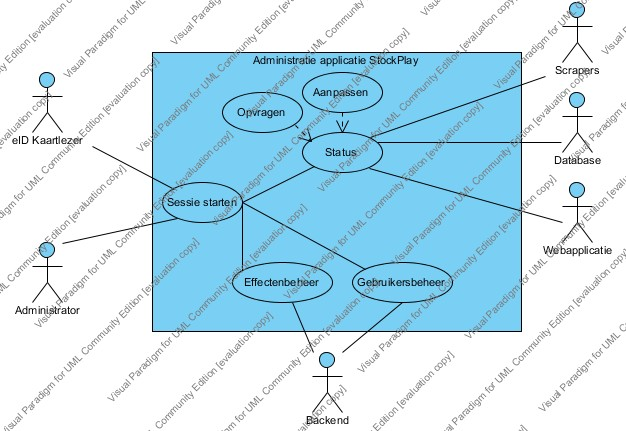
\includegraphics[width=0.5\textwidth]{images/analyse/ucd_desktop}
	\caption{Use-case diagram van de desktopapplicatie.}
\end{figure}

\paragraph{Inloggen van gebruiker}
\begin{compact}
\subparagraph{Beschrijving} Een gebruiker logt in op de desktopapplicatie via zijn e-ID.
\subparagraph{Doel} De administrator is ingelogd op de desktopapplicatie en kan het spel nu beheren.
\subparagraph{Triggers}De gebruiker opent de dekstopapplicatie.
\subparagraph{Prioriteit}Gemiddeld
\subparagraph{Complexiteit}Gemiddeld
\subparagraph{Primaire actoren}Gebruiker, e-ID kaartlezer
\subparagraph{Secundaire actoren}Back-end, databank
\subparagraph{Successcenario}
\begin{enumerate_compact}
 \item De gebruiker krijgt een inlogscherm te zien.
 \item De applicatie vraagt de gebruiker om zijn identiteitskaart in de e-ID lezer te plaatsen en wacht tot dit voltooid is.
 \item De gebruiker plaatst zijn identiteitskaart in de e-ID lezer.
 \item De gebruiker krijgt een voortgangsbalk te zien.
 \item De applicatie leest de nodige gegevens van de identiteitskaart uit.
 \item Er wordt een aanvraag via XML-RPC gestuurd naar de backend om de gegevens te valideren.
 \item De backend raadpleegt de databank om de lijst van administrators op te halen.
 \item Na controle van de gegevens stuurt de backend een antwoord via XML-RPC naar de desktopapplicatie.
 \item De gebruiker is nu ingelogd en krijgt de statuspagina van de desktopappliactie te zien.
\end{enumerate_compact}
\subparagraph{Alternatieve Scenario's}
\begin{enumerate_compact}
	\item[6.] Als een server niet beschikbaar is wordt een foutboodschap getoond.
	\item[8.] Indien de gebruiker niet geregistreerd staat als een administrator wordt een foutmelding getoond en komt hij terug terecht bij stap 2.
\end{enumerate_compact}
\end{compact}

\paragraph{Status van servers bekijken}
\begin{compact}
\subparagraph{Beschrijving} De administrator kan de onlinestatus van de verschillende servers bekijken op de statuspagina. De administrator kan de servers hier ook beheren.
\subparagraph{Doel} De applicatie toont een paneel met daarin de status van de verschillende servers.
\subparagraph{Triggers}De administrator moet ingelogd zijn en het statusmenu openen.
\subparagraph{Prioriteit}Gemiddeld
\subparagraph{Complexiteit}Laag
\subparagraph{Primaire actoren}Administrator
\subparagraph{Secundaire actoren}Back-end, databank
\subparagraph{Successcenario}
\begin{enumerate_compact}
 \item De administrator opent het statusmenu.
 \item De desktopapplicatie vraagt de backend om de status van de verschillende servers te controleren.
 \item De applicatie toont een paneel met de status van de servers samen met mogelijke acties die de administrator kan ondernemen.
 \item In het menu worden snelkoppelingen naar uitgebreidere statuspagina's getoond.
\end{enumerate_compact}
\subparagraph{Alternatieve Scenario's}
\begin{enumerate_compact}
	\item[2.] Als de backend niet antwoord wordt deze als offline beschouwd en krijgen de andere servers als status ``onbekend''.
	\item[4.] Indien de servers niet bereikbaar zijn, zijn deze koppelingen uitgegrijsd.
\end{enumerate_compact}
\end{compact}

\paragraph{Gebruikersgegevens wijzigen}
\begin{compact}
\subparagraph{Beschrijving} Een administrator kan gegevens van een gebruiker wijzigen via de desktopapplicatie.
\subparagraph{Doel} De gegevens van de gespecificeerde gebruiker aanpassen in de databank.
\subparagraph{Triggers}De administrator moet ingelogd zijn en het gebruikersbeheermenu openen.
\subparagraph{Prioriteit}Hoog
\subparagraph{Complexiteit}Gemiddeld
\subparagraph{Primaire actoren}Administrator
\subparagraph{Secundaire actoren}Back-end, databank
\subparagraph{Successcenario}
\begin{enumerate_compact}
 \item De administrator opent het gebruikersbeheermenu.
 \item De applicatie vraagt een lijst van recent geregistreerde gebruikers op bij de back-end en ontvangt deze via XML-RPC. Deze lijst wordt getoond aan de gebruiker in de vorm van een tabel.
 \item De administrator past filters toe om de getoonde lijst te beperken tot de gewenste gebruikers.
 \item Alle gebruikers die aan de filter voldoen worden opgehaald uit de databank en de backend stuurt deze terug via XML-RPC.
 \item De administrator kiest een gebruiker uit de tabel en voert de actie ``Gebruiker bewerken'' uit.
 \item Er wordt een modaal venster getoond met daarin alle beschikbare gegevens van de gebruiker. Niet aanpasbare gegevens worden uitgegrijsd.
 \item De administrator brengt de gewenste wijzigen aan en kiest OK.
 \item De nieuwe gegevens worden doorgestuurd naar de backend.
 \item De backend voert de wijzigingen door in de databank.
 \item De administrator komt terug terecht in de tabel gebruikers.
\end{enumerate_compact}
\subparagraph{Alternatieve Scenario's}
\begin{enumerate_compact}
	\item[2/3.] Als de servers niet bereikbaar zijn wordt een gepaste foutboodschap getoond.
	\item[9.] Indien er een fout optreedt bij het aanpassen van de gegevens in de databank wordt hier een melding van getoond en krijgt de administrator de kans om de ongeldige gegevens aan te passen.
\end{enumerate_compact}
\end{compact}

\paragraph{Effect schorsen of verbergen}
\begin{compact}
\subparagraph{Beschrijving} Als er problemen zijn met een bepaald effect kan een administrator deze schorsen om het verhandelen ervan onmogelijk te maken. Eventueel kan het effect ook onzichtbaar gemaakt worden.
\subparagraph{Doel} Het effect is nu niet meer verhandelbaar in het spel, of is onzichtbaar gemaakt
\subparagraph{Triggers}De administrator is ingelogd en bevindt zich in het effectenbeheermenu
\subparagraph{Prioriteit}Hoog
\subparagraph{Complexiteit}Laag
\subparagraph{Primaire actoren}Administrator
\subparagraph{Secundaire actoren}Back-end, databank
\subparagraph{Successcenario}
\begin{enumerate_compact}
 \item De administrator opent het effectenbeheermenu.
 \item De applicatie toont alle beschikbare effecten in een tabel samen met hun belangrijkste gegevens.
 \item De administrator kan desgewenst een filter toepassen om de lijst te beperken.
 \item De administrator selecteert \'e\'en of meerdere effecten die hij wil aanpassen.
 \item De actie ``Effect(en) verbergen'' of ``Effect(en) schorsen'' wordt gekozen.
 \item De veranderingen worden doorgestuurd naar de backend en deze past de databank aan.
\end{enumerate_compact}
\subparagraph{Alternatieve Scenario's}
\begin{enumerate_compact}
	\item[2.] Als de servers niet bereikbaar zijn wordt een gepaste foutboodschap getoond.
\end{enumerate_compact}
\end{compact}

\paragraph{Gebruiker verbannen}
\begin{compact}
\subparagraph{Beschrijving} Een administrator kan een gebruiker voor een bepaalde tijdsduur uit het spel verbannen.
\subparagraph{Doel} De verbannen gebruiker kan niet meer inloggen gedurende de opgegeven tijdsduur.
\subparagraph{Triggers}De administrator is ingelogd en opent het gebruikersbeheermenu
\subparagraph{Prioriteit}Hoog
\subparagraph{Complexiteit}Laag
\subparagraph{Primaire actoren}Administrator
\subparagraph{Secundaire actoren}Back-end, databank
\subparagraph{Successcenario}
\begin{enumerate_compact}
 \item De administrator opent het gebruikersbeheermenu.
 \item De applicatie krijgt een beperkte lijst van gebruikers die het ontvangt vanuit de back-end.
 \item De administrator past filters toe om de getoonde lijst te beperken tot de gewenste gebruikers.
 \item Alle gebruikers die aan de filter voldoen worden opgehaald uit de databank en de backend stuurt deze terug via XML-RPC.
 \item De administrator selecteert de gewenste gebruikers en kiest voor ``Gebruiker deactiveren''.
 \item Er wordt een venster getoond met daarin de mogelijkheid om een tijdsduur in te geven of een checkbox die aangeeft dat deze gebruiker permanent moet verbannen worden.
 \item De wijzigingen worden gestuurd naar de backend en deze past de gebruikers aan in de databank.
 \item De administrator krijgt opnieuw het gebruikersoverzicht te zien.
\end{enumerate_compact}
\subparagraph{Alternatieve Scenario's}
\begin{enumerate_compact}
	\item[2/4.] Een foutmelding wordt getoond als de backend niet bereikbaar is.
\end{enumerate_compact}
\end{compact}

\paragraph{Schorsen van een effect}
\begin{compact}
\subparagraph{Beschrijving} Een effect dat geschorst is op de beurs kan niet meer verhandeld worden. Dus het kan gekocht noch verkocht worden.
\begin{itemize_compact}
	\item De scraper haalt de JSON-feed op van de website en verwerkt hem
  \item Voor elke opgehaalde koers wordt een XML-RPC-aanroep naar de backend gestuurd met alle gegevens uit de opgehaalde gegevens
  \item De order-verwerking wordt gestart
  \item In de JSON-feed zit ook een timeout-veld. De scraper wacht met de volgende ophaling tot de opgelegde timeout verstreken is
\end{itemize_compact}
\subparagraph{Precondities} De administrator 
\subparagraph{Postcondities} De effect is geschorst
\subparagraph{Prioriteit}Laag
\subparagraph{Complexiteit}Laag
\end{compact}


\subsection{Backend}

\paragraph{Scrapen van beurskoersen}
\begin{compact}
\subparagraph{Beschrijving} De beurskoersen die in dit spel worden gebruikt worden constant live gescraped van enkele beurswebsites
\begin{itemize_compact}
	\item De scraper haalt de JSON-feed op van de website en verwerkt hem
  \item Voor elke opgehaalde koers wordt een XML-RPC-aanroep naar de backend gestuurd met alle gegevens uit de opgehaalde gegevens
  \item De order-verwerking wordt gestart
  \item In de JSON-feed zit ook een timeout-veld. De scraper wacht met de volgende ophaling tot de opgelegde timeout verstreken is
\end{itemize_compact}
\subparagraph{Precondities} De beurs is open
\subparagraph{Postcondities} De huidige koersen zijn in de database opgeslagen
\subparagraph{Prioriteit}Hoog
\subparagraph{Complexiteit}Hoog
\end{compact}

\paragraph{Omzetten van orders naar transacties}
\begin{compact}
\subparagraph{Beschrijving} Als een gebruiker een aandeel wil kopen of verkopen moet hij daar een order voor aanmaken. De effectieve uitvoering van een order gebeurt dan door de beurs zelf. In dit spel gebeurt dit door de backend. Deze controleert elke minuut of de condities voor het order voldaan zijn, en voert deze uit indien ze in orde zijn.
\begin{itemize_compact}
	\item Alle orders worden opgevraagd
  \item Voor elke order gebeuren dan de volgende stappen:
	\begin{itemize_compact}
		\item De condities opgegeven in het order worden gecontroleerd (heeft de koers de opgegeven waarde bereikt, is het effect niet geschorst, etc)
		\item De order wordt uit het systeem verwijderd
		\item De transactie wordt in het systeem ingegeven
	\end{itemize_compact}
\end{itemize_compact}
\subparagraph{Precondities} De beurs is open 
\subparagraph{Postcondities} De orders waarvan de condities voldaan zijn, werden omgezet naar effectieve transactie.
\subparagraph{Prioriteit}Matig
\subparagraph{Complexiteit}Matig
\end{compact}


%
% Functieanalyse
%

\section{Functieanalyse}

\todo{Hier komt een beschrijving van de omgeving waarin het systeem moet werken}


% Ontwerp
\part{Ontwerp}
%
% Functioneel
%

\chapter{Functioneel ontwerp}

\section{Actoren}

\paragraph{Gebruikers}Een gebruiker wordt ge\"identificeerd door een gebruikersnaam en wachtwoord, en wordt intern gelinkt aan een set van rechten, die bepalen wat de gebruiker allemaal kan doen. Zo kennen we de volgende types gebruikers, die elk een verschillende set rechten toegekend worden:
\begin{itemize}
	\item{\emph{Speler}: een gebruiker die deelneemt aan het spel. Hij kan hiervoor gebruik maken van de interactieve delen van de website en van een client op een mobiele telefoon.}
	\item{\emph{Administrator}: deze gebruiker beheert het spel. Hij kan de gebruikers en effecten in het spel beheren, de status van de verschillende componenten bekijken en statistieken raadplegen.}
	\item{\emph{Scraper}: deze gebruiker kan enkel beurzen, index, en aandelen bekijken en aanpassen, en zal dus gebruikt worden door de "scraper" om in het systeem in te loggen en data te pushen naar de database.}
	\item{\emph{Computer}: deze gebruiker neemt, net zoals de "Speler", een deel aan het spel, maar wordt niet bestuurd door een mens maar door een artifici\"ele intelligentie. Dit onderscheid is nodig aangezien een AI extra informatie nodig heeft (zoals het gedrag van andere spelers) om van te leren.}
\end{itemize}

\paragraph{Informaticasystemen}Deze applicatie maakt gebruik van een software design pattern: de 'Three-tier architecture'. De applicatie heeft 3 tiers:
\begin{enumerate}
	\item\emph{Data tier}: Dit is de database waar alle persistente informatie uit het spel wordt in opgeslagen
	\item\emph{Application tier} (ook wel 'Business Logic' genoemd): In deze applicatie wordt deze tier verzorgd door de 'backend'. De backend fungeert als een interface rond de database. Want ze voert alle acties uit op de persistente data in het spel (bijvoorbeeld het aanmaken gebruiker, opslaan \& uitvoeren van orders, ..). Indien de bovenliggende lagen persistente informatie willen opvragen, gebeurt dit ook via deze laag. De communicatie tussen backend en zijn clients gebeurt met behulp van het XML-RPC protocol. 
	\item\emph{Presentation tier}: Deze tier presenteert de informatie aan de eindgebruikers, en laat toe om deze te manipuleren. Alle uitgevoerde manipulaties worden pas effectief als ze zijn doorgegeven aan en uitgevoerd door de Application tier.
De presentation tier bestaat hier uit 3 onafhankelijke applicaties:
	\begin{enumerate}
		\item{de administratieapplicatie}
		\item{de spelwebsite}
		\item{de mobiele spelclient}
	\end{enumerate}
\end{enumerate}
\begin{figure}[h!]
	\centering
		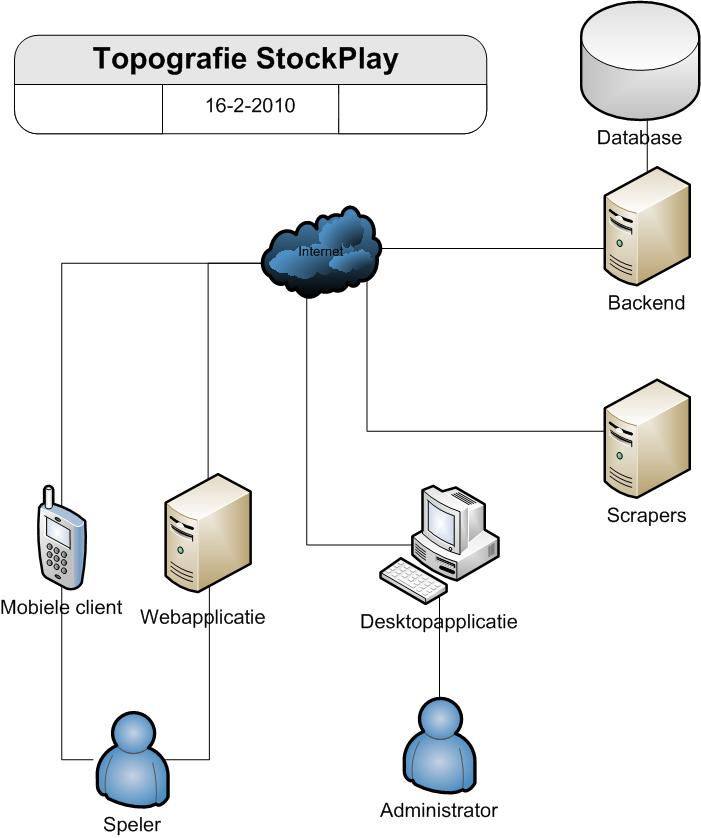
\includegraphics[width=0.5\textwidth]{images/ontwerp/topografie}
	\caption{Topografie van de verschillende systemen.}
\end{figure}

\subparagraph{Scrapers}
StockPlay gebruikt de echte reële beurs, waardoor de koersen van deze effecten moeten dus periodiek worden opgehaald om het spel te laten werken. Hiervoor maken we gebruik van in Perl geschreven scrapers die vanaf enkele vooraf bepaalde internetsites de koersen extraheren. (zoals \makeurl{De Tijd}{http://www.tijd.be/beurzen/euronext-brussel/continumarkt} of \makeurl{Beursduivel}{http://www.beursduivel.be/koersen-belmid.index}).
De opgehaalde informatie wordt vervolgens doorgestuurd naar de backend dewelke deze koersinformatie vervolgens opslaat in de database.

\subparagraph{Atrifici\"ele intelligentie}

Dit zijn computergestuurde spelers, die via het backend-protocol rechtstreeks communiceren met de backend om zo een competitieve medespeler te vormen.


\section{Uitwerking User interfaces}

\subsection{Webapplicatie}

\begin{figure}[h!]
	\centering
		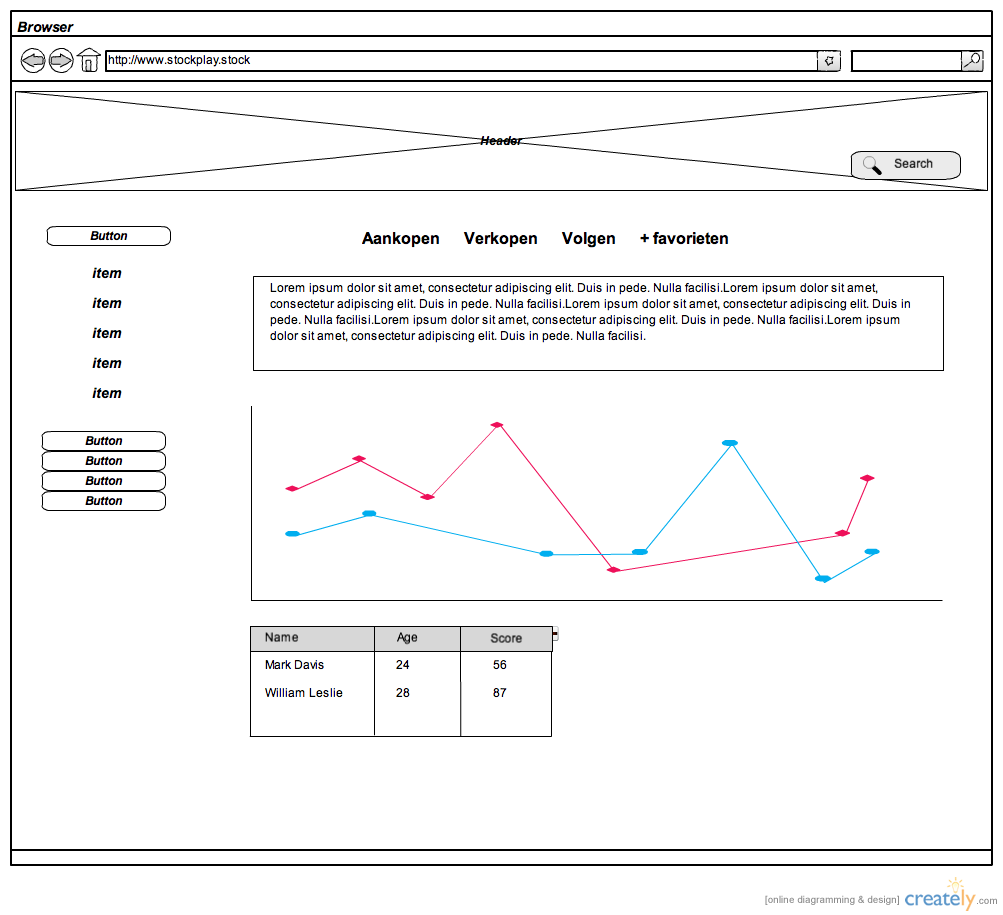
\includegraphics[width=0.5\textwidth]{images/ontwerp/screenshot_website}
	\caption{Layout van de website.}
\end{figure}

Deze interface wordt gebruik om deel te nemen aan het spel. Een gebruiker surft hierbij naar de server die de interface host, en krijgt zo de spelomgeving te zien, dit zonder eerst aan bepaalde softwarevereisten (zoals een Java runtime) te moeten voldaan hebben. Een deel van de functionaliteit is beperkt tot geregistreerde gebruikers.

\paragraph{De algemene overzichtspagina}
Deze pagina geeft de gebruiker een zicht over:
\begin{itemize}
	\item{de huidige waarde van de aangekochte effecten en de meer- of minwaarde op de aankoopprijs}
	\item{zijn cashpositie}
	\item{het totaal van zijn cashpositie en de huidige waarde van de effecten}
	\item{het huidige rendement}
	\item{een grafiek met een overzicht van hun rendement ten opzichte van het gemiddeld rendement, beste rendement, enz.}
	\item{het algemeen klassement en eventuele tussenklassementen}
\end{itemize}

\paragraph{Portfolio}
Vervolgens kan de gebruiker zijn portfolio bekijken, en daar volgende informatie uit halen:
\begin{itemize}
	\item{een overzicht van het portfolio van de gebruiker}
	\item{de effecten momenteel in bezit, aankoopprijs (per stuk en in totaal), huidige koers, rendement en winst/verlies op het aandeel}
\end{itemize}

\paragraph{Overzicht beschikbare effecten}
Er is ook een pagina die een zicht biedt op alle effecten aanwezig in het spel.
\subparagraph{Filters} Om het overzicht te behouden voorziet dat overzicht in verschillende filters:
\begin{itemize}
  \setlength{\itemsep}{1pt}
  \setlength{\parskip}{0pt}
  \setlength{\parsep}{0pt}
	\item{per beurs}
	\item{per type (aandeel, tracker, ...)}
	\item{per index}
	\item{per naam}
	\item{aandelen die als favoriet zijn gekenmerkt door de gebruiker}
	\item{per prijs}
	\item{per volume}
\end{itemize}
\subparagraph{Details per effect}Per aandeel kan vervolgens doorgeklikt worden naar een overzichtspagina, die de volgende informatie biedt:
\begin{itemize}
  \setlength{\itemsep}{1pt}
  \setlength{\parskip}{0pt}
  \setlength{\parsep}{0pt}
	\item{grafiek met koers}
	\item{hoog/laag van de dag}
	\item{huidige koers}
	\item{openingskoers}
	\item{verschil}
	\item{omzet}
	\item{mogelijkheid om te kopen/te verkopen}
\end{itemize}

\paragraph{Transactiegeschiedenis}De gebruiker kan ook een overzicht bovenhalen waarop zijn transactiegeschiedenis zichtbaar is. 
\subparagraph{Details per transactie}Ook hier kan men steeds doorklikken naar een detailpagina in kwestie:
\begin{itemize}
  \setlength{\itemsep}{1pt}
  \setlength{\parskip}{0pt}
  \setlength{\parsep}{0pt}
	\item{het tijdstip}
	\item{het effect}
	\item{het type transactie}
	\item{het aantal}
	\item{de kostprijs voor de transactie}
	\item{de winst/verlies door transactie}
	\item{totaal van uw portefeuille}
\end{itemize}
\subparagraph{Filters}Het overzicht kan worden behouden met behulp van volgende filters:
\begin{itemize}
  \setlength{\itemsep}{1pt}
  \setlength{\parskip}{0pt}
  \setlength{\parsep}{0pt}
	\item{enkel aankopen/verkopen}
	\item{enkel met winst/verlies}
\end{itemize}

\paragraph{Klassementen}Er zijn ook verschillende klassementen aanwezig:
\begin{itemize}
  \setlength{\itemsep}{1pt}
  \setlength{\parskip}{0pt}
  \setlength{\parsep}{0pt}
	\item{meest aangekochte aandelen}
	\item{meest verkochte aandelen}
	\item{spelers top 20 (waarde Portfolio)}
	\item{spelers top 20 (puntentotaal)}
\end{itemize}

\paragraph{Verhandelpagina effecten}De interface voorziet ook in een pagina om aandelen te kopen of verkopen. Hiervoor zijn verschillende mogelijkheden:
\begin{itemize}
  \setlength{\itemsep}{1pt}
  \setlength{\parskip}{0pt}
  \setlength{\parsep}{0pt}
	\item{de prijs die je biedt voor het aandeel. Pas als het aandeel die koers bereikt wordt het aandeel effectief aangekocht}
	\item{de hoeveelheid aandelen die je wenst aan te kopen}
	\item{de max. geldigheidsduur van dit order (1 uur/dag/week/maand)}
\end{itemize}
Tijdens de aankoop krijgt de gebruiker een overzicht van de totale kostprijs en de verschillende taksen die erop staan.

\subsection{Desktopapplicatie}
Deze applicatie voorziet in het beheer van het hele systeem. De beheerder logt daarvoor in met behulp van zijn eID.
De desktopapplicatie is opgesplitst in drie grote componenten.

\paragraph{Systeemstatus}Het laatste grote deel van de applicatie biedt een overzicht van de systeemstatus. Daarbij kan de beheerder het volgende ondernemen:
\begin{itemize}
\item{status van de componenten (scraper, database, website, ...) en starten/stoppen/herstarten van degene die dit aankunnen.}
\item{statistieken bekijken}
	\begin{itemize}
	\item{aantal ingeschreven gebruikers sinds de start}
	\item{aantal gebruikers online}
	\item{aantal connecties per tijdseenheid op de backend}
	\item{aantal transacties per tijdseenheid}
	\item{aantal (succesvol/gefaalde/...) gescrapede aandelen per tijdseenheid}
	\end{itemize}
\end{itemize}

\begin{figure}[h!]
	\centering
		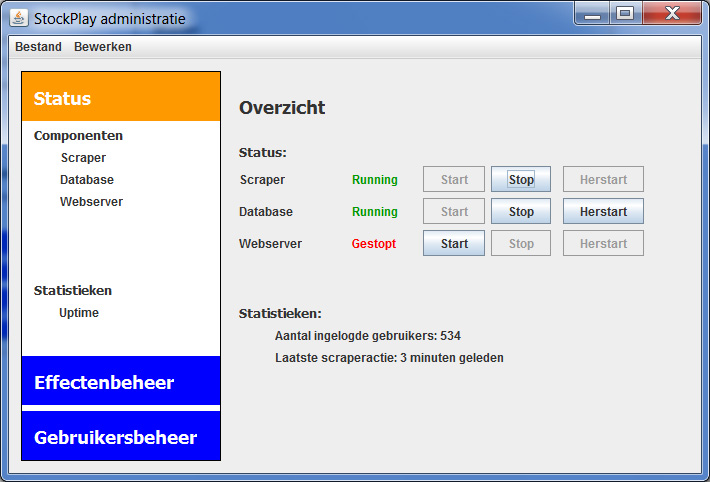
\includegraphics[width=0.5\textwidth]{images/ontwerp/screenshot_app_status}
	\caption{Screenshot van concept statuspagina.}
\end{figure}

\paragraph{Effectenbeheer}Er is ook een overzicht van de effecten voorzien, die de volgende functionaliteit biedt:
\begin{itemize}
	\item{aanduiden van welke effecten moeten gescraped worden, welke effecten zichtbaar zijn bij de spelers}
	\item{schorsen van handel in een effect}
	\item{wijzigen van de gescrapede gegevens}
	\item{overzicht van de aanwezigheid in portefeuilles bij spelers}
\end{itemize}

\begin{figure}[h!]
	\centering
		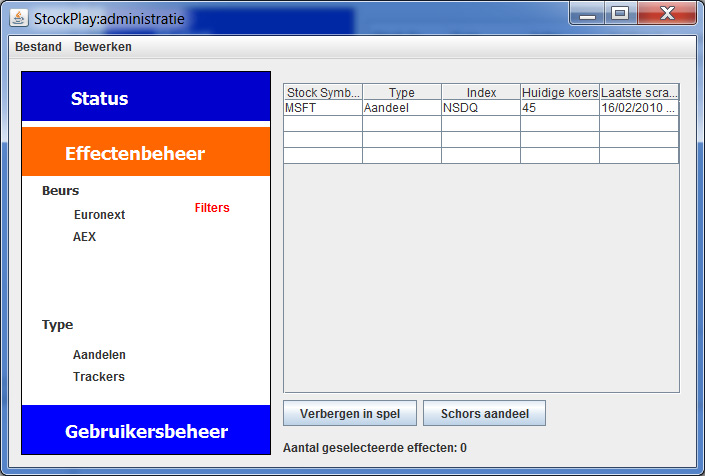
\includegraphics[width=0.5\textwidth]{images/ontwerp/screenshot_app_effecten}
	\caption{Screenshot van concept effectenbeheer.}
\end{figure}

\paragraph{Gebruikersbeheer}Enerzijds is er het overzicht van de gebruikers. Per gebruiker zijn de volgende beheersopdrachten mogelijk: 
\begin{itemize}
	\item{wijzigen van een gebruiker}
	\item{verwijderen van een gebruiker}
	\item{aanpassen van Portfolio: kopen/verkopen van effecten}
	\item{de hoeveelheid cash van de gebruiker aanpassen}
\end{itemize}

\begin{figure}[h!]
	\centering
		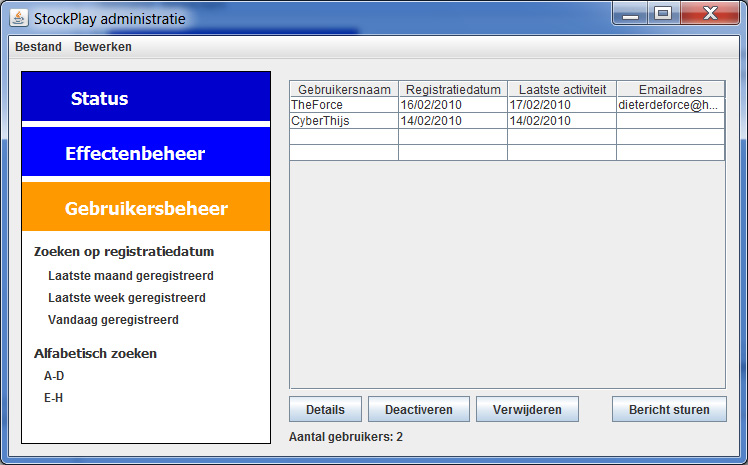
\includegraphics[width=0.5\textwidth]{images/ontwerp/screenshot_app_gebruikers}
	\caption{Screenshot van concept gebruikersbeheer.}
\end{figure}


%
% Technisch
%

\chapter{Technisch ontwerp}

\section{Hergebruik}

\subsection{Backend protocol}

Om toegang te krijgen tot de backend vanuit de verschillende andere delen van het project (zoals de scraper, AI, of interfaces) moesten we op zoek naar een goed communicatieprotocol die aan verschillende vereisten moet voldoen:
\begin{itemize}
\item{taalonafhankelijk: aangezien de interfaces met behulp van verschillende programmeertalen gerealiseerd worden, moet de interface toegankelijk zijn vanuit verschillende programmeertalen.}
\item{lichtgewicht: voor de communcicatie met onze mobiele interface, moet de gegenereerde data compact gehouden worden.}
\item{toegankelijk: de interfaces moeten toegankelijk zijn vanaf een andere machine dan die waar de backand op draait.}
\end{itemize}

Zo hebben we een aantal protocollen overwogen:
\begin{itemize}
\item{een eigen binair protocol}
\item{RMI}
\item{SOAP}
\item{XML-RPC}
\end{itemize}

Het binair protocol viel nogal snel af, aangezien lastig is om te implementeren, relatief foutgevoelig is, en geen garanties biedt qua toegankelijkheid. RMI was ons niet toegestaan te gebruiken, waardoor nog twee kandidaten overbleven: SOAP en XML-RPC. Bij het vergelijken van beide bleek SOAP nogal zwaarwichtig te zijn, en bovendien veel te uitgebreid voor onze (relatief eenvoudige) eisen.

Zo hebben we uiteindelijk gekozen voor het XML-RPC protocol. Dit is een lichtgewicht Remote Procedure protocol, die methodeaanvragen en -antwoorden verpakt in XML-data en ze als POST request verstuurd over het HTTP protocol (zie ook bijlage \ref{chap:xml-rpc} voor de specificaties).
Het protocol voldoet ook aan de opgestelde eisen: aangezien het verder bouwt op het bestaande HTTP-protocol kan het gebruik maken van diens mogelijkheden (zoals compressie en encryptie) en kan het (indien een specifieke bibliotheek onbestaande zou zijn) eenvoudig verwerkt worden met behulp van reeds bestaande HTTP- en XML-bibliotheken. Bovendien verschilt de communicatie niet van regulier HTTP-verkeer waardoor de toegankelijkheid in gelimiteerde netwerkomgevingen ook toeneemt.

Voor de programmeertalen die we gaan gebruiken bij het implementeren bleken er reeds verschillende bibliotheken beschikbaar te zijn, wat het gemak van gebruik opnieuw verhoogt. Een opsomming van de specifieke bibliotheken die we zullen gebruiken om informatie te versturen en ontvangen over het XML-RPC protocol:
\begin{itemize}
\item{\textbf{Perl}: \makeurl{XML::RPC}{http://search.cpan.org/dist/XML-RPC/}}
\item{\textbf{C\#}: \makeurl{XML-RPC.NET}{http://www.xml-rpc.net/}}
\item{\textbf{Java}: \makeurl{Apache XML-RPC}{http://ws.apache.org/xmlrpc/}}
\item{\textbf{Java ME}: \makeurl{kXML-RPC}{http://kxmlrpc.sourceforge.net/}}
\end{itemize}

Deze keuzes zijn eveneens voorzichtig gemaakt. Zo kent Perl nog verschillende andere XML-RPC bibliotheken (zoals de officiële \makeurl{RPC::XML}{http://search.cpan.org/dist/RPC-XML/} bibliotheek), waarvan XML::RPC verschilt in het beperkt aantal afhankelijkheden. Om XML-RPC te gebruiken in Java zijn er ook alternatieven, zoals de \makeurl{Redstone XML-RPC bibliotheek}{http://xmlrpc.sourceforge.net/} die afviel door .... Voor C\# en Java.ME hebben we geen alternatieve bibliotheken gevonden.

\section{Dynamische grafieken}

Op de internetwebsite zullen we een extra module ontwikkelen waarin grafieken dynamisch gemanipuleerd kunnen worden. De gebruikers zullen met eenvoudige muishandelingen andere grafische weergaven van de grafieken kunnen opvragen, zonder de pagina te herladen. Hiervoor zal gebruik gemaakt worden van de interpreter taal Javascript en de javascript bibliotheken \makeurl{JQuery}{http://jquery.com/} en \makeurl{Flot}{http://code.google.com/p/flot/}. JQuery is benodigd om de Flot bibliotheek werkend te krijgen en kunnen we ook op andere plaatsen op de website gebruiken. Deze bibliotheek gaat wat extra functies aan de HTML-elementen hangen en geeft onze eenvoudige middelen om met AJAX extra informatie op te halen.

We gebruiken Flot omdat aan deze bibliotheek nog acief ontwikkeld wordt. Alsook is ze heel eenvoudig gehouden en kan je er makkelijk op voortbouwen. Je kan er op voortbouwen door de ingebouwde events op te vangen en door gebruik te maken van de ingebouwde plugin functionaliteit. Er is ook ondersteuning voor datumweergave en er zijn plugins waarmee je een selectievenster op de grafiek kan activeren (om in te zoomen) en om de grafiek te kunnen verslepen.
De grafieken worden getekend met een combinatie van HTML elementen en het CANVAS element. De HTML elementen kunnen we gemakkelijk vormgeven met CSS. Canvas wordt geëmuleerd in Internet Explorer. Alsook kunnen we de grafieken van deze bibliotheek op een eenvoudige manier vullen met JSON.

\section{Hardware}

\todo{Een vermelding van de mobiele interface}

% Realisatie
\part{Realisatie}
%
% Dataontwerp
%

\chapter{Dataontwerp}

\begin{figure}[h!]
	\centering
		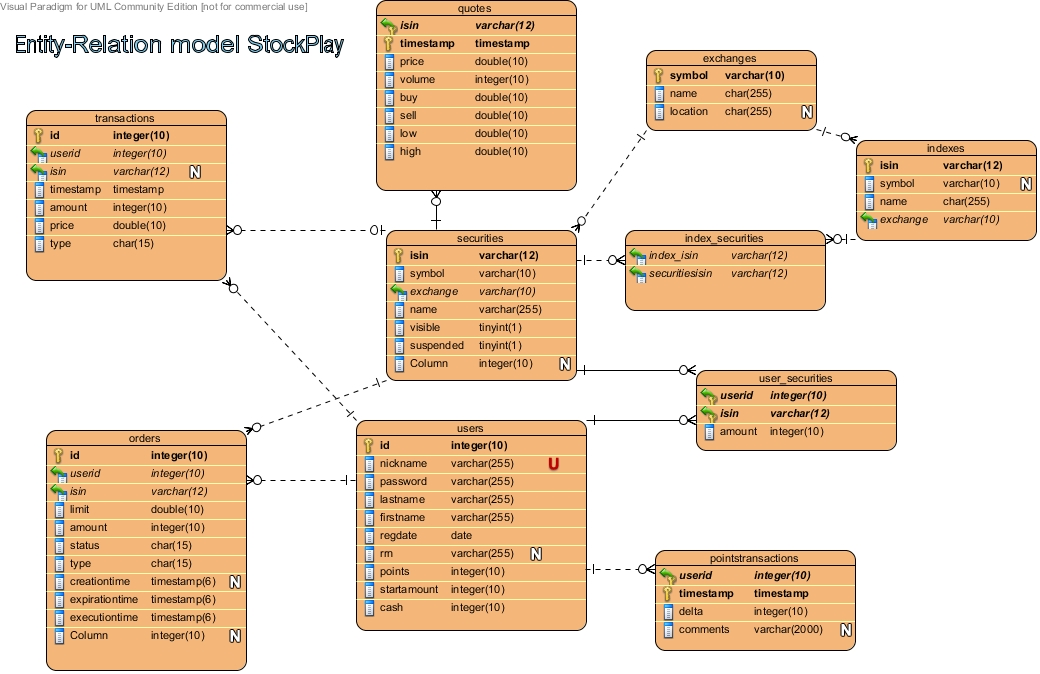
\includegraphics[width=0.5\textwidth]{images/realisatie/ER_Diagram}
	\caption{Entity-relationship model.}
\end{figure}

\section{Afscheiding datatoegang}

Door het gebruik van een aparte backend, wordt rechtstreekse toegang tot de effectieve data verhinderd. Zo kunnen we doorgedreven controles en verificatie van de ingegeven data toepassen, alsook eventuele optimalisaties doorvoeren. Onderstaand diagram illustreert de samenwerking van de componenten in kwestie:

\begin{figure}[h!]
	\centering
		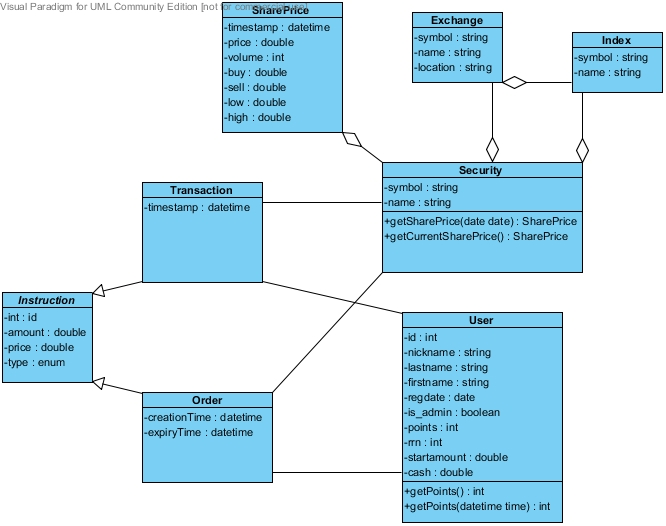
\includegraphics[width=0.5\textwidth]{images/realisatie/Class_Diagram}
	\caption{Overzicht werking backend}
\end{figure}

Op onze databank hebben we ook een aantal triggers. De punten mogen niet zomaar mogen aangepast in de gebruikerstabel. Elke wijziging gebeurt via de pointshistory tabel. Het toevoegen van een nieuw record daarin zorgt ervoor dat een trigger de delta waarde in de pointshistory optelt bij de punten in de userstabel. Zodoende hebben we een cache van het puntentotaal die we snel kunnen raadplegen.

Ook bij het omzetten van een order naar een transactie wordt een trigger geactiveerd die nakijkt of de gebruiker wel voldoende cash positie bezit.

De cash positie van een gebruiker kan niet zomaar aangepast worden, dit wordt ook beveiligd met een trigger.


%
% Procedureontwerp
%

\chapter{Procedureontwerp}

\section{XML-RPC interface}

Zoals vermeld bij het technisch ontwerp, gebruiken we het XML-RPC protocol als communicatiemiddel tussen de backend en zijn interfaces. Hiertoe moeten we de set aan functies vastleggen die een client kan uitvoeren, en de bijhorende signatuur documenteren.

Aangezien XML-RPC geen ondersteuning biedt voor namespaces of andere vormen van functieorganisatie, hanteren we zelf een mechanisme om dit te bekomen: een methode-naam bestaat altijd uit meerdere delen, gescheiden door een punt. De delen voor het scheidingsteken duiden de ``klasse'', het deel erna de methode die we willen oproepen.
Zo delen we de backend op in de volgende drie primaire klassen:
\begin{itemize_compact}
\item{\emph{System}: functionaliteit voor beheer en de statusinformatie van het systeem.}
\item{\emph{User}: beheer van gebruikers en ophalen gebruikersinformatie.}
\item{\emph{Finance}: functionaliteit gerelateerd aan het beurswezen.}
\end{itemize_compact}

\subsection{Algemene foutcodes}

De XML-RPC specificatie biedt ook ondersteuning voor foutberichten, in de form van een bericht met een $<$fault$>$ tag. Die tag moet steeds twee $<$member$>$ tags bevatten, namelijk een foutcode $<$faultCode$>$ van het integer type, en een foutbericht $<$faultString$>$ van het string type.

De mogelijke foutberichten die de backend kan opwerpen, zijn ondergedeeld in verschillende klassen. Bij elke klasse valt de foutcode dan in een specifiek vooraf-gedefini\"eerd bereik, zodat client-software eenvoudig kan detecteren om welk soort fout het gaat. De exacte foutcode, eveneens op voorhand vastgelegd, bepaald vervolgens exacat welke fout er opgeworpen is. Zie tabel \ref{tbl:real:xmlrpc:fouten} voor de mogelijke fouten.
Bij elk type fout gaat zo een standaard foutbericht gepaard, maar de backend-ontwikkelaar kan die eventueel vervangen door een meer specifieke foutmelding.

Om meer informatie over een specifieke fout te bekomen, moet naar de log van de backend gekeken worden. Daar wordt telkens de exacte ``stacktrace'' vermeld, zodat de fout eenvoudig te verhelpen wordt. Een speciaal type fout tenslotte, is de ``internal exception''. Deze treedt op wanneer een exceptie onverwacht optrad, en dus niet in een correcte try-catch blok opgevangen werd.

\begin{table}
\begin{tabular}{| c p{4cm} p{7cm} |}
	\hline
	Foutcode & Foutbericht & Opmerking \\
	\hline
	
	0 & Internal Failure & Een ``untrapped exception'', niet opgevangen door een correcte try-catch clause. \\
	\hline
	
	$[1-10[$ & \emph{Subsystem failures.} & \\
	1 & Database Failure & Er is een probleem met de database (onbeschikbaar, corrupt, ...), zie de log voor meer details. \\
	2 & Scraper Failure & Er is een probleem met de scraper (onbeschikbaar, uitgevallen, ...), zie de log voor meer details. \\
	\hline
	
	$[10-20[$ & \emph{Service exceptions.} & \\
	10 & Service Unavailable & De backend kan tijdelijk niet gebruikt worden (werkzaamheden, overloaded, ...). \\
	11 & Unauthorized & De huidige gebruiker is niet geautoriseerd om de functie in kwestie uit t voeren. \\
	12 & Invalid Credentials & De poging om aan te melden is mislukt, wegens een verkeerde username-password combinatie. \\
	13 & Session Corrupt & De meegeleverde sessie is niet geregistreerd in de backend (verlopen of corrupt). \\
	14 & Not Enough Information & Er is niet genoeg informatie om het object aan te maken (meestal betekent dit dat er een veld in de meegeleverde struct ontbreekt). \\
	\hline
	
	$[20-30[$ & \emph{Invocation issues.} & \\
	20 & Version Not Supported & De client gebruikt een verkeerd communicatieprotocol. \\
	21 & Not Found & Methode niet gevonden, verifieer de schrijfwijze en de klasse. \\
	22 & Bad Request & Probleem met de parameters, controleer het gebruik van de methode. \\
	23 & Non Existing Entity & Het item dat je opvroeg bestaat niet \\
	24 & Pre Existing Entity & Er bestaat reeds zo'n item \\
	25 & Read Only Key & Er is een aanvraag gedaan om een key aan te passen die niet aangepast mag worden \\
	26 & Key does not exist & Er is een aanvraag gedaan om een key aan te passen die niet bestaat \\
	\hline

	$[30-40[$ & \emph{Filter issues.} & \\
	31 & Filter Failure & Er is een probleem met de doorgegeven filter, controleer deze. \\
	32 & Debug Failure & De backend is er niet in geslaagd een debug-AST te genereren van de filter, is de benodigde software ge\"installeerd? \\
	33 & Filter Failure & De backend slaagde er niet in twee filters samen te smelten om een resultaatset-reductie te bekomen. \\
	
	\hline
\end{tabular}
\caption{Mogelijke fouten binnen het backend-protocol.}
\label{tbl:real:xmlrpc:fouten}
\end{table}

\subsection{Authenticatie en autorisatie}

Aangezien het XML-RPC protocol gebruik maakt van het HTTP-protocol, kunnen we diens functionaliteit gebruiken om authenticatie te bekomen. Daartoe zullen we gebruik maken van \emph{basic authentication}, waarbij de client indien gevraagd een gebruikersnaam en wachtwoord naar de server doorstuurd. Normaal zou dit geen extra code teweegbrengen, en zouden we volledig op de authenticatiemogelijkheden van het HTTP protocol kunnen berusten.

Deze denkpiste gaf echter enkele problemen. Vooreerst is het sterk onveilig aangezien het wachtwoord continu in (quasi) plaintext doorgestuurd wordt. Het maakt echter verfijnde autorisatie moeilijk, tenzij we voor elk authenticatie-niveau een aparte URL zouden voorzien. Daarom hebben we gekozen om gebruik te maken van een eigen authenticatie-laag, waarbij een XML-RPC functie gebruikt wordt om de gebruiker aan te melden (dit in tegenstelling tot het gebruik maken van de HTTP laag). Na aanmelding geeft de functie in kwestie een sessie-ID terug, die een sessie serverside linkt aan een specifieke gebruiker. Zo kunnen we, opnieuw binnenin de XML-RPC laag, controleren of een gebruiker wel correct aangemeld is, en heel dynamisch requests toelaten of weigeren. Dit is gebaseerd op een flexibel rechten-systeem, waarbij elke gebruiker in de database gelinkt wordt aan een rol die bepaalde rechten toekent.

Om de veiligheid te verhogen gebruiken we verschillende technieken. Eerst en vooral is de sessie tijdelijk, en worden ongebruikte sessie-keys regelmatig geinvalideerd. Ook hebben we het moeilijk gemaakt om sessie-keys te genereren, door ze op een unieke manier te linken aan data die enkel de gebruiker zelf kent (zijn wachtwoord). Om het tenslotten ook moeilijk te maken om een sessie-key te linken aan een gebruiker, implementeren we in onze sessie-hash een variabele seed.

Authenticatie en autorisatie gaat ook gepaard met een specifieke set aan mogelijke errormessages. Allemaal geklasseerd binnen de Service Exceptions, zijn de volgende subtypes mogelijk: ``Invalid Credentials'' wanneer het authenticeren mislukt is, ``Unauthorized'' wanneer een gebruiker niet geautoriseerd is tot het gebruik van een bepaalde functie, en tenslotte ``Session Corrupt'' wanneer een gespecificeerde sessie ongeldig blijkt te zijn (zie tabel \ref{tbl:real:xmlrpc:fouten}).

De mogelijke autorisatieniveau's zijn beschreven in tabel \ref{tbl:real:xmlrpc:autorisatie}. Hoewel een administrator deze bij gebruikers manueel kan aanpassen, onderscheiden we toch volgende categorie\"en:
\begin{itemize_compact}
\item{Gast}
\item{Speler}
\item{Administrator}
\item{Scraper}
\end{itemize_compact}

\begin{table}
\begin{tabular}{| c p{7cm} |}
	\hline
	Autorisatie-niveau & Beschrijving \\
	\hline
	
	BACKEND\_ADMIN & Administrator rechten voor methodes betreffende de backend. \\
	DATABASE\_ADMIN & Administrator rechten voor methodes betreffende de database. \\
	SCRAPER\_ADMIN & Administrator rechten voor methodes betreffende de scraper. \\
	POINTS\_ADMIN & Administrator rechten voor methodes betreffende het puntenbeheer. \\
	TRANSACTION\_ADMIN & Administrator rechten voor methodes betreffende het transactie-beheer. \\
	
	SECURITY\_UPDATE & Toegang tot methodes die effecten updaten (toevoegen van quotes). \\
	SECURITY\_CREATE & Toegang tot methodes die nieuwe effecten aanmaken. \\
	SECURITY\_REMOVE & Toegang tot methodes die effecten verwijderen. \\
	SECURITY\_MODIFY & Toegang tot methodes die effecten wijzigen. \\
	
	USER\_REMOVE & Toegang tot methodes die gebruikers verwijderen. \\
	
	LOGGEDIN & Standaard-recht voor ingelogde gebruikers. \\
	NONE & Standaard recht voor iedereen (ook gasten). \\
	
	\hline
\end{tabular}
\caption{Autorisatieniveau's binnen het backend-protocol.}
\label{tbl:real:xmlrpc:autorisatie}
\end{table}

\subsection{System klasse}

Deze klasse biedt de client mogelijkheden om het systeem te beheren. Zoals het ophalen van informatie, wijzigen van configuraties, en (her)starten of stoppen van bepaalde subsystemen.

\subsubsection{Backend subklasse}

\function{Backend.Status}
	{ status van de backend ophalen }
	{ geen }
	{ integer die de status beschrijft:
		\begin{itemize_compact}
		\item{0: maintenance-mode}
		\item{1: functioneert normaal}
		\end{itemize_compact} }
	{ BACKEND\_ADMIN }

\function{Backend.Stats}
	{ backend-statistieken ophalen }
	{ geen }
	{ struct met statistieken:
		\begin{itemize_compact}
		\item{users: aantal gebruikers online}
		\item{req: aantal verwerkte XML-RPC requests sinds de start van de backend}
		\item{uptime: hoe lang de backend al draait}
		\end{itemize_compact} }
	{ BACKEND\_ADMIN }

\function{Backend.Restart (NIET GE\"IMPLEMENTEERD)}
	{ de backend opnieuw opstarten }
	{ geen }
	{ bool die indiceert of de actie succesvol was }
	{ BACKEND\_ADMIN }

\function{Backend.Stop (NIET GE\"IMPLEMENTEERD)}
	{ de backend stoppen }
	{ geen }
	{ bool die indiceert of de actie succesvol was }
	{ BACKEND\_ADMIN }

\function{Backend.ClearCache}
	{ de backend cache legen }
	{ geen }
	{ bool die indiceert of de actie succesvol was }
	{ BACKEND\_ADMIN }


\subsubsection{Database subklasse}

\function{Database.Status}
	{ informatie van de database ophalen }
	{ geen }
	{ integer die status beschrijft:
		\begin{itemize_compact}
		\item{0: er kon geen verbinding naar de databank gelegd worden}
		\item{1: succesvol verbonden met de database}
		\end{itemize_compact} }
	{ DATABASE\_ADMIN }

\function{Database.Stats}
	{ database-statistieken ophalen. Dit zijn de statistieken geleverd door de databank zelf, ze zijn dus niet beperkt tot acties ondernomen door de backend }
	{ geen }
	{ struct met statistieken:
		\begin{itemize_compact}
		\item{uptime: hoe lang de databank al draait}
		\item{rate: aantal transacties per seconde}
		\end{itemize_compact} }
	{ DATABASE\_ADMIN }


\subsubsection{Scraper subklasse}

\function{Scraper.Status (NIET GE\"IMPLEMENTEERD)}
	{ status van de scraper ophalen }
	{ geen }
	{ integer die status beschrijft:
		\begin{itemize_compact}
		\item{0: niet geactiveerd}
		\item{1: inactief}
		\item{2: bezig met data-mining}
		\end{itemize_compact} }
	{ SCRAPER\_ADMIN }

\function{Scraper.Stats (NIET GE\"IMPLEMENTEERD)}
	{ scraper-statistieken ophalen }
	{ geen }
	{ struct met statistieken:
		\begin{itemize_compact}
		\item{executes: aantal voltooide plugin-uitvoeringen}
		\item{uptime: hoe lang de scraper al draait}
		\item{traffic: hoeveelheid data verzonden en ontvangen}
		\item{plugins: aantal geactiveerde plugins}
		\item{securities: aantal beschikbare effecten}
		\item{exchanges: aantal beschikbare beurzen}
		\item{indexes: aantal beschikbare indexen}
		\item{delay: tijd tot de volgende plugin-uitvoering}
		\item{memory: geheugengebruik}
		\end{itemize_compact} }
	{ SCRAPER\_ADMIN }

\function{Scraper.Restart (NIET GE\"IMPLEMENTEERD)}
	{ de scraper herstarten }
	{ geen }
	{ bool die indiceert of de actie succesvol was }
	{ SCRAPER\_ADMIN }

\function{Scraper.Stop (NIET GE\"IMPLEMENTEERD)}
	{ de scraper permanent stilleggen }
	{ geen }
	{ bool die indiceert of de actie succesvol was }
	{ SCRAPER\_ADMIN }


\subsection{User klasse}

Hier vindt men de nodige methodes terug om gebruikers te beheren. Dit is echter niet beperkt tot de administrator: ook gebruikers zelf kunnen hun eigen profiel (in beperktere mate) beheren.

\function{Hello}
	{ protocolcontrole uitvoeren }
	{ de naam van de applicatie (string), en het nummer van de protocolimplementatie (int) }
	{ een boolean die aangeeft of de actie al dan niet gelukt is, of een exceptie indien de vermelde protocolversie niet ondersteund wordt }
	{ NONE }
	
\function{Validate}
	{ controleren van user credentials en genereren van een sessie-ID }
	{ de gebruikersnaam (string) en wachtwoord (string) }
	{ een sessie-ID voor verder gebruik, of een exceptie indien het aanmelden mislukt is }
	{ NONE }
		
\function{CreateSessionForUser}
	{ manueel een sessie cre\"eren voor verder gebruik }
	{ de user-id waarvoor een sessie moet gecre\"eerd worden }
	{ een sessie-ID voor verder gebruik }
	{ BACKEND\_ADMIN }

\function{List}
	{ lijst met publieke informatie opvragen van de gebruikers }
	{ een filter om gebruikers te selecteren, met de volgende mogelijke sleutels:
		\begin{itemize_compact}
		\item{id: de ID van de gebruiker}
		\item{nickname: gebruikersnaam}
		\item{firstname: de voornaam van de gebruiker}
		\item{lastname: de achternaam van de gebruiker}
		\item{rrn: het rijksregisternummer van de gebruiker}
		\item{email: het e-mailadres van de gebruiker}
		\item{regtime: datum van registratie}
		\item{cash: de hoeveelheid cash die de gebruiker effectief bezit}
		\item{points: aantal behaalde punten}
		\end{itemize_compact} }
	{ een lijst met oppervlakkige gebruikersinformatie (in de vorm van een struct):
		\begin{itemize_compact}
		\item{id: gebruikers-id}
		\item{nickname: gebruikersnaam}
		\item{cash: de hoeveelheid cash die de gebruiker effectief bezit}
		\item{regdate: datum van registratie}
		\item{startamount: het kapitaal waarmee de gebruiker begonnen is}
		\item{points: aantal behaalde punten}
		\item{role: een verwijzing naar de rollen die de gebruiker beoefent}
		\end{itemize_compact} }
	{ NONE }

\function{Details}
	{ lijst met publieke informatie opvragen van een gebruiker }
	{ een filter om gebruikers te selecteren, zie de List functie }
	{ een lijst met gedetailleerde gebruikersinformatie (in de vorm van een struct):
			\begin{itemize_compact}
			\item{id: gebruikers-id}
			\item{nickname: gebruikersnaam}
			\item{firstname: de voornaam van de gebruiker}
			\item{lastname: de achternaam van de gebruiker}
			\item{email: het e-mailadres van de gebruiker}
			\item{cash: de hoeveelheid cash die de gebruiker effectief bezit}
			\item{regdate: datum van registratie}
			\item{rrn: het rijksregisternummer van de gebruiker}
			\item{startamount: het kapitaal waarmee de gebruiker begonnen is}
			\item{points: aantal behaalde punten}
			\item{role: een verwijzing naar de rollen die de gebruiker beoefent}
			\end{itemize_compact} }
	{ BACKEND\_ADMIN }
	
\function{Details}
	{ publieke informatie opvragen van de gebruiker zelf }
	{ geen (de filter wordt impliciet geconfigureerd op een selectie van details van de huidige gebruiker) }
	{ idem als Details aanroep met een filter }
	{ LOGGEDIN }

\function{Create}
	{ aanmaken van een nieuwe gebruiker }
	{ struct met de gebruikersinformatie:
		\begin{itemize_compact}
		\item{nickname: gebruikersnaam}
		\item{firstname: de voornaam van de gebruiker}
		\item{lastname: de achternaam van de gebruiker}
		\item{email: het e-mailadres van de gebruiker}
		\item{rrn: het rijksregisternummer van de gebruiker}
		\item{role: een verwijzing naar de rollen die de gebruiker beoefent}
		\end{itemize_compact} }
	{ id van de aangemaakte gebruiker }
	{ NONE }

\function{Modify}
	{ wijzigen van een bestaande gebruiker }
	{ een filter die gebruikers selecteert, en een struct met de te-wijzigen gebruikersinformatie:
		\begin{itemize_compact}
			\item{nickname: gebruikersnaam}
			\item{firstname: de voornaam van de gebruiker}
			\item{lastname: de achternaam van de gebruiker}
			\item{email: het e-mailadres van de gebruiker}
			\item{rrn: het rijksregisternummer van de gebruiker}
			\item{role: een verwijzing naar de rollen die de gebruiker beoefent}
		\end{itemize_compact} }
	{ een boolean die aangeeft of de actie al dan niet gelukt is }
	{ BACKEND\_ADMIN }

\function{Modify}
	{ wijzigen van de gebruiker zelf }
	{ idem als Modify aanroep met een filter, maar zonder een filter (die impliciet geconfigureerd wordt zodat de wijziging enkel van toepassing is op de huidige gebruiker) }
	{ idem als Modify aanroep met een filter }
	{ LOGGEDIN }

\function{Remove}
	{ verwijderen van een bestaande gebruiker }
	{ een filter die gebruikers selecteert, zie de List aanroep }
	{ een boolean die aangeeft of de actie al dan niet gelukt is }
	{ USER\_REMOVE }
	
\function{ResetPassword}
	{ publieke informatie opvragen van de gebruiker zelf }
	{ de gebruikersnaam (string), en het nieuwe wachtwoord (string) }
	{ idem als Details aanroep met een filter }
	{ NONE (wegens tijdsgebrek, zou in een later stadium strikter gecontroleerd worden) }


\subsubsection{Portfolio subklasse}

\function{Portfolio.List}
	{ basisinformatie van effecten in bezit opsommen (gebruik vervolgens functie Finance.Security.Details voor meer informatie) }
	{ een filter, met de volgende mogelijke sleutels:
		\begin{itemize_compact}
		\item{id: een gebruikers-id}
		\end{itemize_compact} }
	{ array van structs met basisinformatie van de effecten:
		\begin{itemize_compact}
		\item{isin: identificatiecode van het aandeel}
		\item{amount: het aantal aandelen in bezit van de gebruiker}
		\item{user: het ID van de gebruiker in kwestie}
		\end{itemize_compact} }
	{ BACKEND\_ADMIN, of LOGGEDIN (maar dan wordt de resultaatset gereduceerd tot portfolio van de ingelogde gebruiker) }

\function{Portfolio.Create}
	{ een nieuw effect toevoegen aan de portfolio van een gebruiker (praktisch wordt dit meestal gerealiseerd met triggers) }
	{ een struct met de volgende sleutels:
		\begin{itemize_compact}
		\item{isin: identificatiecode van het aandeel}
		\item{amount: het aantal aandelen in bezit van de gebruiker}
		\item{user: het ID van de gebruiker in kwestie}
		\end{itemize_compact} }
	{ een boolean die aangeeft of de actie al dan niet gelukt is }
	{ TRANSACTION\_ADMIN }


\subsubsection{Order subklasse}

\todo{behoudt Orders.List ook uitgevoerde orders van een bepaald timeframe? - we hadden normaal gezegd dat we hier alle order tonen, ook de uitgevoerde. Het timeframe/resente orders zetten is dan kwestie van het zetten van de juiste filter en kan de client dan zelf bepalen. Kan je je hier in vinden? - Laur}
\function{Order.List}
	{ wachtende orders bekijken }
	{ een filter, met de volgende mogelijke sleutels:
		\begin{itemize_compact}
		\item{id: id van het order}
		\item{userid: id van de gebruiker}
		\item{isin: identificatiecode van het aandeel}
		\item{amount: het aantal effecten dat het aandeel verhandelt}
		\item{type: het type order}
		\item{creationtime: het moment waarop het order aangemaakt is}
		\item{expirationtime: het moment waarop het order vervalt}
		\item{executiontime: het moment waarop het order uitgevoerd is}
		\item{secondairylimit (sic): de secundaire limiet}
		\item{status: de status van het order}
		\end{itemize_compact} }
	{ lijst van structs met order-informatie:
		\begin{itemize_compact}
		\item{id: id van het order}
		\item{user: id van de gebruiker}
		\item{type: het type order}
		\item{isin: identificatiecode van het aandeel}
		\item{amount: het aantal aandelen dat aangekocht worden}
		\item{status: de status van het order}
		\item{creationtime: het moment waarop het order aangemaakt is}
		\item{expirationtime: het moment waarop het order vervalt}
		\item{executiontime: het moment waarop het order uitgevoerd is}
		\item{secondairylimit (sic): de secundaire limiet}
		\end{itemize_compact} }
	{ BACKEND\_ADMIN (moet ooit ORDER\_ADMIN worden), of LOGGEDIN (maar dan wordt de resultaatset gereduceerd tot orders van de ingelogde gebruiker) }

\todo{specifieke foutmelding als order aanmaken faalde}
\function{Order.Create}
	{ een nieuw order aanmaken }
	{ struct met orderdetails
		\begin{itemize_compact}
		\item{user: id van de gebruiker}
		\item{isin: identificatiecode van het aandeel}
		\item{type: het type order}
		\item{amount: het aantal aandelen dat aangekocht worden}
		\item{status: de status van het order}
		\item{creationtime: het moment waarop het order aangemaakt is}
		\item{expirationtime: het moment waarop het order vervalt}
		\item{executiontime: het moment waarop het order uitgevoerd is}
		\item{secondairylimit (sic): de secundaire limiet}
		\end{itemize_compact} }
	{ id van het aangemaakte order }
	{ BACKEND\_ADMIN (moet ooit ORDER\_ADMIN worden), of LOGGEDIN (indien het 'id' veld in de ingegeven struct overeenstemp met die van de ingelogde gebruiker) }

\function{Order.Cancel}
	{ een bestaande order annuleren }
	{ een filter (zie Order.List) }
	{ geen }
	{ BACKEND\_ADMIN (moet ooit ORDER\_ADMIN worden), of LOGGEDIN (maar dan wordt de set waarop de functie inwerkt gereduceerd tot orders van de ingelogde gebruiker) }

\function{Order.Modify}
	{ een bestaande order wijzigen }
	{ een filter die orders selecteert (zie Order.List), en een struct met de te-wijzigen orderinformatie:
		\begin{itemize_compact}
		\item{type: het type order}
		\item{amount: het aantal aandelen dat aangekocht worden}
		\item{status: de status van het order}
		\item{creationtime: het moment waarop het order aangemaakt is}
		\item{expirationtime: het moment waarop het order vervalt}
		\item{executiontime: het moment waarop het order uitgevoerd is}
		\item{secondairylimit (sic): de secundaire limiet}
		\end{itemize_compact} }
	{ geen }
	{ BACKEND\_ADMIN (moet ooit ORDER\_ADMIN worden), of LOGGEDIN (maar dan wordt de set waarop de functie inwerkt gereduceerd tot orders van de ingelogde gebruiker) }


\subsubsection{Transaction subklasse}

\function{Transaction.List}
	{ lijst van uitgevoerde transacties weergeven }
	{ een filter, met de volgende mogelijke sleutels:
		\begin{itemize_compact}
		\item{id: identificatie van de transactie}
		\item{userid: identificatie van de gebruiker}
		\item{timest: datum van uitvoering}
		\item{isin: identificatiecode van het effect}
		\item{type: type verhandeling}
		\item{amount: aantal verhandelde effecten}
		\item{price: prijs waarvoor het aandeel verhandeld is}
		\item{comments: commentaar bij de verhandeling}
		\end{itemize_compact} }
	{ array van structs die transactie-informatie bevatten:
		\begin{itemize_compact}
		\item{amount: aantal verhandelde effecten}
		\item{id: identificatie van de transactie}
		\item{user: identificatie van de gebruiker}
		\item{time: datum van uitvoering}
		\item{isin: identificatiecode van het effect}
		\item{type: type verhandeling}
		\item{price: prijs waarvoor het aandeel verhandeld is}
		\item{comments: commentaar bij de verhandeling}
		\end{itemize_compact} }
	{ TRANSACTION\_ADMIN, of LOGGEDIN (maar dan wordt de set waarop de functie inwerkt gereduceerd tot orders van de ingelogde gebruiker) }

\textbf{Opmerking}: bij deze methode is geen verschil gemaakt tussen een reguliere List en een Details opvraging, aangezien de methode enkel kan aangeroepen worden door geautoriseerde gebruikers.

\function{Transaction.Create}
	{ nieuwe transactie aanmaken }
	{ struct met transactie-details:
		\begin{itemize_compact}
		\item{amount: aantal verhandelde effecten}
		\item{user: identificatie van de gebruiker}
		\item{time: datum van uitvoering}
		\item{isin: identificatiecode van het effect}
		\item{type: type verhandeling}
		\item{price: prijs waarvoor het aandeel verhandeld is}
		\item{comments: commentaar bij de verhandeling}
		\end{itemize_compact} }
	{ id van de aangemaakte transactie }
	{ TRANSACTION\_ADMIN }

\function{Transaction.Modify}
	{ nieuwe transactie aanmaken }
	{ een filter die transacties selecteert (zie List), en een struct met de te-wijzigen transactieinformatie:
		\begin{itemize_compact}
		\item{amount: aantal verhandelde effecten}
		\item{time: datum van uitvoering}
		\item{isin: identificatiecode van het effect}
		\item{type: type verhandeling}
		\item{price: prijs waarvoor het aandeel verhandeld is}
		\item{comments: commentaar bij de verhandeling}
		\end{itemize_compact} }
	{ id van de aangemaakte transactie }
	{ TRANSACTION\_ADMIN }


\subsubsection{Points subklasse}

\function{Points.List}
	{ lijst van transactie-punten ophalen }
	{ een filter, met de volgende mogelijke sleutels:
		\begin{itemize_compact}
		\item{userid: gebruikers-id}
		\item{timest: datum van uitvoering}
		\item{delta: verandering van het puntenaantal door deze transactie}
		\item{comments: commentaar bij de verhandeling}
		\end{itemize_compact} }
	{ array van structs die transactiepunt-informatie bevatten:
		\begin{itemize_compact}
		\item{userid: gebruikers-id}
		\item{timestamp: datum van uitvoering}
		\item{delta: verandering van het puntenaantal door deze transactie}
		\item{comments: commentaar bij de verhandeling}
		\end{itemize_compact} }
	{ POINTS\_ADMIN, of LOGGEDIN (maar dan wordt de set waarop de functie inwerkt gereduceerd tot orders van de ingelogde gebruiker) }

\function{Points.CreateTransaction}
	{ nieuwe transactie aanmaken op het huidige moment }
	{ struct met transactie-details:
		\begin{itemize_compact}
		\item{user: gebruikers-id}
		\item{delta: verandering van het puntenaantal door deze transactie}
		\item{comments: commentaar bij de verhandeling}
		\end{itemize_compact} }
	{ id van de aangemaakte transactie }
	{ TRANSACTION\_ADMIN }

\function{Points.DeleteTransaction}
	{ bestaande transactie verwijderen }
	{ een object, dat de waarden bevat van de transactie die verwijderd moeten worden:
		\begin{itemize_compact}
		\item{user: gebruikers-id}
		\item{delta: verandering van het puntenaantal door deze transactie}
		\item{comments: commentaar bij de verhandeling}
		\item{timestamp: de tijd van verhandeling}
		\end{itemize_compact} }
	{ boolean die indiceert of het verwijderen succesvol was }
	{ TRANSACTION\_ADMIN }

\function{Points.Ranking}
	{ ranking ophalen van een bepaalde groep gebruikers }
	{ een filter die een groep gebruikers selecteer (zie Users.List) }
	{ een array van structs, die Rank objecten voorstellen:
		\begin{itemize_compact}
		\item{id: gebruikers-id}
		\item{total: het aantal punten dat de gebruiker heeft}
		\item{rank: de rank van de gebruiker}
		\end{itemize_compact} }

\huge DIETER VUL DIT AAN, WAT DOET Points.EventRanking? EN CONTROLEER Points.Ranking OOK!
\normalsize
		

\subsection{Finance klasse}

Tenslotte zijn er nog de methodes gerelateerd met het effectieve beurswezen, die (hoofdzakelijk) terug te vinden zijn in deze klasse. Enkel het ophalen van de portfolio bevindt zich, logischerwijs, in de User-klasse.

\subsubsection{Exchange subklasse}

\function{Exchange.List}
	{ lijst van beurzen opvragen }
	{ een filter, met de volgende mogelijke sleutels:
		\begin{itemize_compact}
		\item{symbol: de symbool van de beurs}
		\item{name: de naam van de beurs}
		\item{location: de locatie van de beurs}
		\end{itemize_compact} }
	{ array van structs met beurs-info:
		\begin{itemize_compact}
		\item{symbol: de symbool van de beurs}
		\item{name: de naam van de beurs}
		\item{location: de locatie van de beurs}
		\end{itemize_compact} }
	{ NONE }

\function{Exchange.Modify}
	{ informatie van een beurs wijzigen }
	{ een filter om beurzen te selecteren (zie Exchange.List), en een struct met beursinformatie:
		\begin{itemize_compact}
		\item{name: de naam van de beurs}
		\item{location: de locatie van de beurs}
		\end{itemize_compact} }
	{ niks }
	{ SECURITY\_MODIFY }

\function{Exchange.Create}
	{ een beurs toevoegen }
	{ een struct met beursinformatie:
		\begin{itemize_compact}
		\item{symbol: de symbool van de beurs}
		\item{name: de naam van de beurs}
		\item{location: de locatie van de beurs}
		\end{itemize_compact} }
	{ niks }
	{ SECURITY\_CREATE }


\subsubsection{Index subklasse}

\function{Index.List}
	{ lijst van indexen opvragen }
	{ een filter, met de volgende mogelijke sleutels:
		\begin{itemize_compact}
		\item{name: de naam van de index}
		\item{exchange: het symbool van de beurs waarop de index zich bevindt}
		\item{isin: het identificatiesymbool van de index}
		\item{symbol: het symbool van de index}
		\end{itemize_compact} }
	{ array van structs met index-informatie:
		\begin{itemize_compact}
		\item{name: de naam van de index}
		\item{exchange: het symbool van de beurs waarop de index zich bevindt}
		\item{isin: het identificatiesymbool van de index}
		\item{symbol: het symbool van de index}
		\end{itemize_compact} }
	{ NONE }

\function{Index.Modify}
	{ informatie van een index wijzigen }
	{ een filter, en een struct met indexinformatie:
		\begin{itemize_compact}
		\item{name: de naam van de index}
		\end{itemize_compact} }
	{ niks }
	{ SECURITY\_MODIFY }

\function{Index.Create}
	{ een index toevoegen }
	{ en een struct met indexinformatie:
		\begin{itemize_compact}
		\item{name: de naam van de index}
		\item{exchange: het symbool van de beurs waarop de index zich bevindt}
		\item{isin: het identificatiesymbool van de index}
		\item{symbol: het symbool van de index}
		\end{itemize_compact} }
	{ niks }
	{ SECURITY\_CREATE }


\subsubsection{Security subklasse}

\function{Security.List}
	{ lijst met oppervlakkige informatie van effecten opvragen }
	{ een filter, met de volgende mogelijke sleutels:
		\begin{itemize_compact}
		\item{symbol: het symbool van het effect}
		\item{name: de naam van het effect}
		\item{exchange: de beurs waarop het effect zich bevindt}
		\item{visible: een bool die beschrijft of het aandeel zichtbaar is}
		\item{suspended: een bool die indiceert of het aandeel geschorst is}
		\item{isin: identificatiecode van het effect}
		\end{itemize_compact} }
	{ array van structs met informatie over het effect:
		\begin{itemize_compact}
		\item{symbol: het symbool van het effect}
		\item{name: de naam van het effect}
		\item{exchange: de beurs waarop het effect zich bevindt}
		\item{visible: een bool die beschrijft of het aandeel zichtbaar is}
		\item{suspended: een bool die indiceert of het aandeel geschorst is}
		\item{isin: identificatiecode van het effect}
		\end{itemize_compact} }
	{ NONE }

\textbf{Opmerking}: ook hier hebben we geen onderscheid gemaakt tussen een List en Details methode, aangezien er niet echt datavelden zijn die niet mogen geraadpleegd worden door niet-geautoriseerde clients.

\function{Security.Modify}
	{ informatie van een effect wijzigen }
	{ een filter (zie Security.List), en een struct met informatie over het effect:
		\begin{itemize_compact}
		\item{name: de naam van het effect}
		\item{visible: een bool die beschrijft of het aandeel zichtbaar is}
		\item{suspended: een bool die indiceert of het aandeel geschorst is}
		\end{itemize_compact} }
	{ aantal aangepaste effecten }
	{ SECURITY\_MODIFY }

\function{Security.Create}
	{ een effect toevoegen }
	{ een struct met informatie over het effect:
		\begin{itemize_compact}
		\item{symbol: het symbool van het effect}
		\item{name: de naam van het effect}
		\item{exchange: de beurs waarop het effect zich bevindt}
		\item{visible: een bool die beschrijft of het aandeel zichtbaar is}
		\item{suspended: een bool die indiceert of het aandeel geschorst is}
		\item{isin: identificatiecode van het effect}
		\end{itemize_compact} }
	{ niks }
	{ SECURITY\_CREATE }
	
\function{Security.Remove}
	{ een effect verwijderen }
	{ een filter (zie Security.List) }
	{ aantal verwijderde effecten }
	{ SECURITY\_REMOVE }

\function{Security.Update}
	{ nieuwe quote aan een security toevoegen }
	{ een struct dat een quote voorstelt, met de volgende inhoud:
		\begin{itemize_compact}
		\item{isin: identificatiecode van het effect}
		\item{time: tijdstip waarop de koers geldt}
		\item{price: huidige koers van het aandeel}
		\item{volume: omzet van het aandeel op de dag in kwestie (cumulatief voor 1 dag)}
		\item{bid: biedprijs van het aandeel}
		\item{ask: vraagprijs van het aandeel}
		\item{low: laagterecord van het aandeel op de dag in kwestie}
		\item{high: hoogterecord van het aandeel op de dag in kwestie}
		\item{open: openingsprijs van het aandeel op de dag in kwestie}
		\end{itemize_compact} }
	{ niks }
	{ SECURITY\_UPDATE }

\function{Security.UpdateBulk}
	{ reeks van nieuwe quotes toevoegen }
	{ vector van structs die voldoen aan de signatuur van Security.Update }
	{ niks }
	{ SECURITY\_UPDATE }

\function{Security.Quotes}
	{ quotes van een aandeel ophalen }
	{ filter, met de volgende mogelijke sleutels:
		\begin{itemize_compact}
		\item{isin: identificatiecode van het effect}
		\item{timestamp: tijd waarop de koers geldde}
		\item{price: huidige koers van het aandeel}
		\item{volume: omzet van het aandeel op de dag in kwestie (cumulatief voor 1 dag)}
		\item{bid: biedprijs van het aandee}
		\item{ask: vraagprijs van het aandee}
		\item{low: laagterecord van het aandeel op de dag in kwestie}
		\item{high: hoogterecord van het aandeel op de dag in kwestie}
		\item{open: openingsprijs van het aandeel op de dag in kwestie}
		\end{itemize_compact} }
	{ array van structs met de koersen van het effect:
		\begin{itemize_compact}
		\item{isin: identificatiecode van het effect}
		\item{time: tijdstip waarop de koers geldt}
		\item{price: huidige koers van het aandeel}
		\item{volume: omzet van het aandeel op de dag in kwestie (cumulatief voor 1 dag)}
		\item{bid: biedprijs van het aandee}
		\item{ask: vraagprijs van het aandee}
		\item{low: laagterecord van het aandeel op de dag in kwestie}
		\item{high: hoogterecord van het aandeel op de dag in kwestie}
		\item{open: openingsprijs van het aandeel op de dag in kwestie}
		\end{itemize_compact} }
	{ NONE }

\function{Security.Quotes}
	{ quotes van een aandeel ophalen, aan een bepaalde resolutie }
	{ 4 argumenten:
		\begin{itemize}
		\item{een datum die het begin van het bereik aanduidt}
		\item{een datum die het eind van het bereik aanduidt}
		\item{een integer die indiceert tot hoeveel punten de resolutie moet geschaald worden}
		\item{een filter (zie Security.Quotes)}
		\end{itemize} }
	{ een array van structs met de koersen van het effect (zie Security.Quotes) }
	{ NONE }

\function{Security.LatestQuotes}
	{ de laatste quotes van bepaalde aandelen ophalen }
	{ een filter die de effecten selecteert (zie Security.Quotes) }
	{ een array van structs met de laatste koersen van het effect (zie Security.Quotes) }
	{ NONE }

\function{Security.QuoteRange}
	{ het bereik van de koersen van een aandeel ophalen }
	{ de identificatiecode van een aandeel (string) }
	{ het bereik, als een vector met twee datums in (start en einde van het bereik) }
	{ NONE }

\function{Security.getHighest}
	{ de hoogste koers van een reeks aandelen ophalen }
	{ een filter die de effecten selecteert (zie Security.Quotes) }
	{ een struct, die de hoogste koers van de selectie voorstelt (zie Security.Quotes) }
	{ NONE }

\function{Security.getLowest}
	{ de laagste koers van een reeks aandelen ophalen }
	{ een filter die de effecten selecteert (zie Security.Quotes) }
	{ een struct, die de laagste koers van de selectie voorstelt (zie Security.Quotes) }
	{ NONE }


\subsubsection{IndexSecurity subklasse}

Deze klasse biedt, zoals de User.Portfolio klasse doet met Users, een link tussen Securities en Indexes.

\function{IndexSecurity.List}
	{ lijst van relaties tussen Indexes en Securities opvragen }
	{ een filter, met de volgende mogelijke sleutels:
		\begin{itemize_compact}
		\item{index\_isin: identificatiesymbool van de index}
		\item{security\_isin: identificatiesymbool van het effect}
		\end{itemize_compact} }
	{ array van structs die relaties uitdrukken:
		\begin{itemize_compact}
		\item{index\_isin: identificatiesymbool van de index}
		\item{security\_isin: identificatiesymbool van het effect}
		\end{itemize_compact} }
	{ NONE }

\function{Security.Create}
	{ een effect toevoegen }
	{ een struct die een relatie uitdrukt tussen een index en een effect:
		\begin{itemize_compact}
		\item{index\_isin: identificatiesymbool van de index}
		\item{security\_isin: identificatiesymbool van het effect}
		\end{itemize_compact} }
	{ niks }
	{ SECURITY\_CREATE }


%
% Grafieken
%

\todo{details over de implementatie van Laurens zijn grafieken. Misschien ook alles van styling (template/masterpage) hier?}

\chapter{Dynamische grafieken}

Zoals reeds vermeld maken we gebruik van de JQuery en FLOT bibliotheken om interactieve grafieken te maken. Die zullen volgende functionaliteit bevatten:
\begin{itemize_compact}
\item{zoomen in de grafiek doormiddel van het scrolwiel}
\item{zoomen in de grafiek doormiddel van een dubbelklik op een locatie}
\item{uitzoomen met een knop}
\item{de grafiek zal je kunnen vastnemen en over de x-as verslepen}
\item{je zal kunnen wisselen tussen een sleepmodus en een modus waarin je een kader kan selecteren waarin je wil inzoomen (enkel over de x-as)}
\item{er zal onderaan een tweede, gekoppelde grafiek te zien zijn waarin een bargrafiek te zien is waar de volumes van de effecten in te zien zijn}
\item{eventueel: je zal extra referentie lijnen kunnen toevoegen}
\item{je zal een beperkt aantal maal op je laatste handelingen kunnen terugkeren}
\item{de opgehaalde punten zullen gecached worden en enkel indien vereist zal via AJAX nieuwe punten opgehaald worden}
\end{itemize_compact}


%
% Scraper
%

\chapter{Scraper}

De scraper is een elementair gedeelte van StockPlay, daar het hele project nood heeft aan een up-to-date dataset.

\section{Databronnen}

Vooraleer een scraper te ontwerpen, was het belangrijk de mogelijke bronnen te identificeren. Logischerwijs beperken we ons tot gratis beschikbare bronnen, maar zelfs dan komen er verschillende bronnen in aanmerking. Om uiteindelijk een zo uitgebreid mogelijke dataset te hebben, besloten we om het mogelijk te maken verschillende bronnen tegelijk te gebruiken.

\subsection{De Tijd}

Een eerste kandidaat om onze scraper op in te laten werken, was de website van De Tijd. Deze site voorziet in een uitgebreid aanbod aandelen en indexen van verschillende beurzen, en biedt sommige van die data zelfs real-time aan. Verder onderzoek van hoe die realtime updates gebeurden - en het reverse-engineering van de bijhorende HTTP-based API - leverde ons nogal snel een compact Perl-script op dat in staat was de aandelen en indexen van een bepaalde beurs eenmalig op te halen, om in een later stadium dan de effectieve koersen op te halen via de aangeboden API in kwestie.

Aangezien deze bron een hele waaier aan aandelen zichtbaar maakt, er veel data over publiceert, en bovendien die data beschikbaar maakt via een compacte en handige interface, hebben we deze als belangrijkste bron gebruikt bij het opvullen en updaten van onze database.

\subsection{Euronext}

Deze offici\"ele bron biedt via een webinterface heel gedetailleerde informatie over alle aandelen die beschikbaar zijn op de beurs. De site biedt ook een ruime blik in het verleden, door de gebruiker toe te laten om 2 jaar aan koersen op te halen. Hoewel deze data veel beter en hi\"erarchischer georganiseerd is, hebben we besloten deze bron niet te gebruiken en de site van De Tijd eerder te gebruiken. De reden hiervoor is dat de site van De Tijd, die eveneens alle aandelen op de Euronext beurs kan weergeven, realtime data weergeeft en hierbij ook een handigere en compactere interface voor gebruikt.

De site bleek echter wel nuttig te zijn bij het ontwerpen van een artifici\"ele intelligentie, waarbij niet zozeer realtime data maar vooral veel historische data benodigd is om het massief-lerende netwerk te trainen.

\subsection{Perl Finance modules}

Het Perl CPAN archief kent een uitgebreid aanbod aan modules die in staat zijn om koersen van aandelen op te halen van verschillende bronnen. Hoewel deze bron uitmunt in gemak van gebruik (eenvoudige maar doordachte API, hergebruik van code) hebben we toch besloten deze niet te gebruiken. De motivatie daarvoor bestaat uit een aantal punten: eerst en vooral is het de bedoeling dat we zelf een Perl scraper schrijven, eenvoudigweg een bestaande module gebruiken voldoet niet aan deze eis. Daarnaast kennen de modules voor Europese beurzen niet dezelfde kwaliteit en resolutie als een zelfgemaakt script die de site van De Tijd of die van Euronext raadpleegt, en een hoge resolutie is belangrijk om een kwalitatief en correct verloop van het spel te garanderen.

\section{Ontwerp}

Om op een flexibele wijze verschillende bronnen parallel te kunnen raadplegen, hebben we geopteerd voor een plugin-based design. Hierbij wordt elke bron geassocieerd met een enkele plugin, die een vaste interface implementeert om gestandaardiseerd data-opvragingen van buitenaf toegankelijk te maken. De plugins kunnen echter ook hi\"erarchisch uitgebreid worden: zo zal een plugin die data ophaalt niet rechtstreeks de \emph{Source} interface implementeren, maar gebruik maken van de \emph{Website} interface, die op zijn beurt de \emph{Source} interface uitbreidt met functionaliteit toegespitst tot websites.

De hoofdinterface Source beschrijft essentieel twee kenmerken: het beschikbaar zijn van een ``exchanges'' attribuut, en een ``getLatestQuotes'' methode. Het \textbf{exchanges} attribuut is een hi\"erarchische structuur van de beurzen die de plugin kan scrapen: de elementen zijn instanties zijn van de StockPlay::Exchange klasse, waarvan de objecten toegang geven tot de indexen (klasse StockPlay::Index) en aandelen (klasse StockPlay::Security) van de klasse. De verantwoordelijkheid voor het aanmaken van deze structuur ligt bij de plugin die het Exchange object aangemaakt heeft.
De Plugin interface dwingt ook een \textbf{getQuotes} functie af, die gebruikt wordt om eenmaal de initi\"ele opbouw aan Exchanges, Securities en Indexen voltooid is, de koersen van een lijst Securities op te halen. Deze functie geeft dan ook een lijst aan StockPlay::Quote objecten terug. Dergelijke objecten, 1 op 1 verbonden met een Security, bevatten de effectieve koersdata. Zo zijn verschillende velden beschikbaar zoals ``time'', ``volume'', of ``price''. Een ander belangrijk veld is het ``delay'' veld, dat omschrijft hoe lang er moet gewacht worden om een nieuwe koers op te halen.

Nu vastligt hoe de data in een uniforme en gestructureerde wijze opgeslagen wordt, is het duidelijk dat de data opgedeeld kan worden in twee categorie\"en: presistente en variabele data.
Onder de persistente data behoort de hi\"erarchie aan Exchange, Security en Index objecten die omschrijft welke beurzen en aandelen de plugin toegang tot heeft, en hoe die zich onderling relateren. Aangezien de objecten in kwestie steeds voorzien in een ``private data container'' (die plugins kunnen gebruiken om bronspecifieke maar verder niet relevante data op te slaan), volstaat het om die eenmaal op te bouwen. Ze kunnen daarna steeds opnieuw herbruikt worden om de variabele data op te halen. Die variabele data bestaat natuurlijk uit de uiteindelijke Quotes.
Door deze essenti\"ele splitsing is het mogelijk om de persistente data eenmaal op te halen en dan binnen een bepaald interval te herbruiken om variabele data op te halen. Dit maakt de scraper niet alleen sneller, het verlaagt ook de hoeveel data die steeds benodigd is om de aangevraagde data op halen. Hierbij reduceren we de kans dat de scraper teveel opvalt en eventueel zou verbannen worden van de bron in kwestie.

Functionaliteit zoals de private data containers, en andere huishoudelijke functionaliteit, zit verpakt in de StockPlay::Plugin klasse. Elke klasse die zich gedraagt als een plugin (zoals de Source interface hierboven beschreven), moeten deze klasse implementeren. Dit onderscheid is gemaakt zodat de plugin manager ook nog gebruikt zou worden voor andere scripts die gebruik maken van het Perl framework dat ontwikkeld is in functie van de scraper, zoals de artifici\"ele intelligentie.

\section{Communicatie}

Nu de scraper in staat is om gevraagde koersen op een effici\"ente manier op te halen, moet de methode van communicatie naar de backend nog ontworpen worden. Hierbij zijn er twee mogelijkheden: een PUSH of PULL model.

In geval van een \textbf{PULL} model is de Backend de initiator, en zal die de scraper vragen om een bepaalde selectie data. In een \textbf{PUSH} model daarentegen zal de scraper zelf het initiatief nemen. Hierbij is het vrij snel duidelijk dat het PUSH model de beste keuze is. Moesten we immers voor een PULL model gaan, dan zou de scraper nog een apart protocol moeten defini\"eren, of in geval van hergebruik van het XML-RPC protocol voorzien in een webserver en XML-RPC decoder. Als we echter voor een PUSH model kiezen, moet de scraper enkel voorzien in een XML-RPC client (wat veel minder werk is), en kan de reeds bestaande XML-RPC server code in de backend integraal herbruikt worden.
Om dit te realiseren zal de backend wel moeten voorzien in speciale functies toegespitst op de werking van de scraper, zoals het toevoegen van aandelen, of updaten van de bijhorende koersen. Ook is deze uitbreiding van het backend-protocol de druppel geweest die ons overtuigde om ten behoeve van autorisatie om te schakelen van een eenvoudige boolean-flag (isAdmin) naar een flexibeler model gebaseerd op rechten.

Om het PUSH model te realiseren moet de scraper voorzien in een algoritme dat continu alle aandelen overloopt, en selectief voor diegene die verlopen zijn nieuwe koersen ophaalt en die naar de backend stuurt. Deze functionaliteit wordt ge\"implementeerd door de StockPlay::Scraper klasse, dewelke bezit over een lijst van de geactiveerde plugins, en zo in de \emph{run()} functie van alle plugins de aandelen ophaalt en ze eventueel vernieuwt. Tijdens de refresh-run wordt tevens bepaald hoelang minimaal moet gewacht worden vooraleer er een nieuwe cyclus kan gestart worden. Om echter de belasting van de databron te minimaliseren, maakt de scraper intelligent gebruik van verschillende statistieken (zoals hoelang geleden het aandeel voor het laatst geüpdatet is) om de berekende wachttijd te transformeren naar een wachttijd passend bij het aandeel in kwestie.


%
% Artifici\"ele intelligentie
%

\chapter{Artifici\"ele intelligentie}

Als illustratie van de modulariteit van de backend, hebben we ook een artifici\"ele intelligentie aangemaakt die het spel meespeelt zoals een reguliere speler dat doet. Dit was echter geen evidente opdracht, en er was flink wat opzoekingswerk benodigd om dit tot een goed einde te brengen.


\section{Intelligentie}

Prioritair om aan de implementatie te kunnen beginnen, was het vinden van een geschikt algoritme die de intelligentie van de speler zou drijven. Hiervoor hebben we verschillende opties overwogen, gaande van expertsystemen zoals regelbanken, tot meer massief-lerende systemen zoals genetische algoritmes of neurale netwerken. Expertsystemen zijn vrij snel afgevoerd, ze werken misschien wel nauwkeurig maar hebben nood aan een uitgebreide set (moeilijk kwantificeerbare) regels die bovendien voor het opstellen een expertise vereisen die geen van ons hebben. Om aan deze eis van expertise te ontsnappen, zijn we gaan kijken naar massief lerende systemen die zichzelf kunnen verbeteren aan de hand van een ruime set aan testgegevens. Hierbij zijn genetische algoritmes misschien wel een interessante piste, maar ze vereisen een vrij specifieke implementatie: een library integreren zou veel werk kosten, laat staan het schrijven van een eigen implementatie. Zo zijn we uitgekomen op neurale netwerken, dewelke uiteindelijk ook eenvoudig integreerbaar bleken te zijn.

Een neuraal netwerk is een populaire methode om artifici\"eel gedrag te bekomen, en baseert zich daarbij op hoe een biologisch brein functioneert. Hierbij wordt dynamisch een gewogen pad gevormd tussen een vast aantal input en output neuronen, en zal via backpropagatie steeds ge\"evolueerd worden in de richting van een correctere oplossing. We hebben er voor gekozen om een aantal gegevens (zoals de koers van het aandeel, de koers van een overkoepelende index, de dag van de week, het volume, etc) als inputneuronen te registreren, en een enkel output neuron vast te leggen als de slotkoers van de volgende dag. Moesten we immers de slot van de volgende dag kunnen bepalen aan de hand van gegevens bepaald op de huidige dag, kunnen we steeds een positief-renderende portfolio samenstellen.

Bij het bepalen van de inputneuronen hebben we ons gebaseerd op bestaande kennis die te vinden was in de verschillende papers die we geraadpleegd hebben bij het kiezen van een optimale intelligentie-algoritme. In de uiteindelijke versie van het project worden de volgende inputs gebruikt:
\begin{itemize}
\item Slotkoers op dag $i$
\item Slotkoers van de meest prominente index op dezelfde beurs op dag $i$
\item Laagste koers van het aandeel op dag $i$
\item Hoogste koers van het aandeel op dag $i$
\item Verkoopvolume van het aandeel op dag $i$
\end{itemize}

Gebaseerd op dergelijke inputinformatie, zal het neuraal netwerk zich werken naar een set van outputdata die volgende informatie bevat:
\begin{itemize}
\item Slotkoers op dag $i+1$
\end{itemize}

Hoewel het ontwerpen van een eenvoudig neuraal netwerk misschien niet zoveel tijd kost, hebben we er voor gekozen om een bestaande bibliotheek te gebruiken. Verschillende belangrijke features die de performantie van het netwerk serieus verbeteren (zoals backpropagatie, shortcut-netwerken, of automatisch bepalen van een ideale activatiefunctie), zijn te moeilijk om binnen het opgegeven tijdsbestek zelf te implementeren. Bovendien is het enkel te bedoeling om de modulariteit van de backend te demonstreren, waaraan het implementeren van ingewikkelde algoritmen nauwelijks bijdraagt.


\section{Omgeving}

Bibliotheken om gebruik te maken van neurale netwerken, zijn wegens performantieredenen meestal geschreven in low-level talen zoals C of C++. Dit zou echter betekenen dat we opnieuw een datalaag zouden moeten opbouwen, en dit terwijl we reeds functionele datalagen hadden in zowel Java, Perl als C\#. Om toch niet in te moeten inboeten aan performantie, hebben we ervoor gekozen om gebruik te maken van een bestaande datalaag, en op zoek te gaan naar een bibliotheek geschreven in een performante taal, die bindings aanbiedt in de taal waarin onze datalaag geschreven is. Hierdoor is het performantieverlies minimaal, en kunnen we toch het schrijven van nog een datalaag vermijden.

Het in Perl geschreven \makeurl{AI::FANN}{http://search.cpan.org/~salva/AI-FANN-0.10/lib/AI/FANN.pm} pakket voldoet volledig aan deze specificatie: we kunnen gebruik maken van de bestaande datalaag die we reeds geschreven hebben voor de scraper, terwijl de echte performantie gehaald wordt door het interfacen met de in C geschreven bibliotheek \makeurl{FANN}{http://leenissen.dk/fann/}. Deze bibliotheek biedt tevens vele geavanceerde mogelijkheden, zoals het automatisch wijzigen van netwerkparameters via een genetisch algoritme, waarbij zowel activatiefuncties als neuronen dynamisch kunnen gewijzigd worden.


\section{Historische data}

Om een massief-lerend systeem te trainen, is er een voldoende hoeveelheid aan historische data nodig. Hierbij moet zowel de input als output waarden bekend zijn, zodat het netwerk via backpropagatie en andere technieken de gewichten van de paden in het netwerk kan bijstellen (of eventueel andere structurele veranderingen toevoegen). Die data hebben we kunnen halen bij de site van Euronext, een bron die we initi\"eel afgekeurd hadden wegens het gebrek aan realtime data, maar nu uitermate handig bleek te zijn door zijn eenvoudige interface tot data die 2 jaar in het verleden teruggaat.


\section{Modulariteit}

Om in een eventueel later stadium toe te laten om op een eenvoudige wijze gebruik te maken van alternatieve algoritmes, hebben we gebruik gemaakt van de plugin-infrastructuur ontwikkeld voor de scraper. Het is heel eenvoudig mogelijk om extra intelligentie-algoritmes toe te voegen, die dynamisch en automatisch zullen gebruikt worden bij het samenstellen van de ideale portfolio. Hierbij wordt elk algoritme steeds gebruikt, en diegene met de kleinste voorspelde fout uiteindelijk gebruikt om de slotkoers van de volgende dag te voorspellen.

Analoog aan hoe we de scraper plugin-infrastructuur gerealiseerd hebben, zal elke voorspellings-plugin  verplicht de interface StockPlay::AI::Forecaster moeten implementeren. Die klasse, die op zijn beurt StockPlay::Plugin implementeert, legt een interface vast die vervolgens door de AI manager kan gebruikt worden om het netwerk te trainen, koersen te voorspellen, foutmarges op te halen, etc. Zo worden uiteindelijk at-runtime alle voorspellers uitgeprobeerd, om uiteindelijk het nauwkeurigste resultaat te gebruiken bij selectie van een portfolio.


\section{Portfolio selectie}

Wanneer er tenslotte slotkoersen voor de volgende dag voorspeld zijn, moet er nog een optimale portfolio samengesteld worden. Dit aspect mag misschien klein lijken, het is helemaal niet evident om dit intelligent te realiseren! Een goed algoritme zou hierbij kijken naar de nauwkeurigheid van elke voorspelling, zich baseren op het uiteindelijke resultaat van vorige voorspellingen, en gebruik maken van vastgelegde parameters die bepalen hoe ``conservatief'' of net ``risicovol'' het zich moet gedragen. Maar dit valt opnieuw ruim buiten de scope van dit project, niet alleen is het geen exacte wetenschap, ook is het een relatief ongedocumenteerd onderwerp en zou er veel tijd kruipen in het ontwikkelen en benchmarken van een dergelijk algoritme. Daarom hebben we geopteerd om een eenvoudig algoritme te gebruiken, waarbij een evenredige selectie genomen wordt van de meest performante aandelen gebaseerd op een enkele voorspelling. Dit opnieuw omdat de artifici\"ele intelligentie vooral ontworpen is om de modulariteit en eenvoudige uitbreidbaarheid van de backend te demonstreren, het ontwikkelen van een complex portfolio-selectiealgoritme is hierbij irrelevant.


%
% Netwerkoptimalisaties
%

\chapter{Netwerkoptimalisaties}

Tijdens de implementatie van de applicatie, zijn we verschillende keren tegen een netwerk-gerelateerde bottleneck gelopen. Zo duurde het in eerste instantie bijvoorbeeld ettelijke seconden vooraleer de backend de laatste quotes van een bepaalde beurs opgehaald had. Om te vermijden dat de gebruiker effectief verschillende seconden moet wachten op het resultaat van een bewerking, hebben we verschillende optimalisaties toegepast.


\section{Datacompressie}

Zoals reeds vermeld bij de voordelen van het XML-RPC protocol, kunnen we eenvoudig gebruik maken van beschikbare technologie\"en. Zo hebben we om de duur van een request te verlagen, gebruik gemaakt van de compressie mogelijkheden die het HTTP-protocol reeds aanbiedt. De client kan zo in een request de \emph{Accept-Encoding} header meesturen, waarop de backend eventueel op gepaste wijze kan reageren door de reply te comprimeren. Hier zijn we echter tegen een beperking van de ws-xmlrpc library gelopen die we gebruiken binnen onze backend: enkel de \emph{gzip} compressietechniek wordt ondersteund. Dit had als gevolg dat we de Perl library \emph{RPC::XML} hebben moeten wijzigen, aangezien die enkel de \emph{deflate} compressietechniek ondersteunt (eigenlijk was dit niet nodig, bij gebrek aan ondersteuning werd compressie niet gebruikt, maar gezien de hoeveelheid data die de scraper dagelijks naar de backend stuurt was compressie toch gewenst).


\section{Caching}

Hoewel de bovenstaande netwerkoptimalisatie een grote impact heeft (grote datatransfers werden met factor 10 versneld), hielp dit niet bij de requests die de backend zelf stuurt in de richting van de database. Die requests zijn mogelijks reeds gecomprimeerd (aangezien ze verlopen via een binair protocol eigen aan de Oracle JDBC driver), maar zorgden toch voor een substanti\"ele vertraging. Zo bleek, na implementatie van datacompressie bij requests en replies, dat een groot deel van de originele delay zijn oorsprong kende bij het ophalen van data uit de database.

Daarom hebben we besloten om de datalaag in de backend uit te breiden met een flexibel caching systeem. Dit resulteerde echter in een aantal interessante problemen: wat moet er juist in de cache, wanneer worden entries geinvalideerd, en hoe bepalen we wat relevant is en wat te vluchtig is om in een cache op te slaan? Veel van deze problemen zijn niet eigen aan ons project, maar vallen binnen het domein van caches. Daarom hebben we besloten om een deel van deze problematiek te elimineren door gebruik te maken van een bestaande caching bibliotheek. De keuze is daarbij gevallen op \makeurl{cache4j}{http://cache4j.sourceforge.net/}: een compacte doch performante caching bibliotheek die net voldoende features biedt om aan onze eisen te voldoen.

De standaard opzet bij caches is om de data die de gebruiker terugkrijgt op te slaan, en wanneer de gebruiker iets opvraagt eerst de cache te controleren. Zo zouden we een cache moeten opzetten met beurzen, aandelen, koersen, etc. Wanneer de gebruiker dan een lijst van de beurzen opvraagt, kunnen we eenvoudigweg de inhoud van de cache teruggeven in plaats van de database te moeten contacteren.
De opzet van ons project bemoeilijkt dit concept echter. Aangezien we gebruik maken van een filter die nooit geïnterpreteerd wordt door de backend, maar louter gecompileerd wordt tot een string die de database dan kan verwerken, heeft de backend nooit weet van wat de effectieve selectiecriteria van de dataset waren. Daarom kunnen we het resultaat van de bevraging niet eenvoudig opslaan, laat staan in een later stadium de cache raadplegen om de juiste entries op te halen.
Om toch een cache te kunnen gebruiken, slaan we geen hiërarchie van datasets op, maar louter het letterlijke antwoord dat een gebruiker zou moeten krijgen bij een specifieke aanvraag. De sleutel die web gebruiken om de resultaatset op te slaan in de cache, is een gemodificeerde content-aware representatie van de aa,vraag, samengesteld uit de methodenaam en de argumentenlijst (meestal een filter). Zo zal een aa,vraag bij de backend, gericht op eenzelfde functie (vb ``Finance.Exchange.List''), waarbij de argumenten inhoudelijk identiek zijn aan de argumenten van een vorige aanroep, niet resulteren in een bevraging bij de database maar louter in het teruggeven van een waarde uit de cache.
Hoewel dit complex mag lijken, valt dit in Java relatief eenvoudig te implementeren. Eerst hebben we voorzien in een Proxy klasse, die elke aanvraag op object kan herleiden via een InvocationHandler (indien caching gewenst is natuurlijk). Die InvocationHandler zal in actie treden wanneer een willekeurige functie aangeroepen wordt op een object dat geregistreerd is bij de Proxy. In die methode kunnen we vervolgens de content-aware hashcode genereren, de cache controleren, eventueel een opgeslagen waarde teruggeven, of indien die ontbrak een aanroep naar het effectieve object uitvoeren om daarna het resultaat in de cache op te slaan.
Om dit proces vervolgens flexibel te maken, hebben we gebruikt van Java annotaties (\emph{@Cachable} en \emph{@Invalidates}), die de programmeur van de Data Access Objecten eenvoudig kan toevoegen aan een functiedeclaratie, om zo de interpretatie binnen een eventuele InvocationHandler te manipuleren.

Zoals vermeld hierboven hebben we ook voorzien in een \emph{@Invalidates} annotatie, die de InvocationHandler duidelijk maakt dat een bepaalde aanroep juist de bijhorende cache invalideert. Om de effici\"entie hierbij te verhogen, hebben we de cache gesplitst in een aantal deelcaches, elk geassocieerd met een specifiek Data Access Object. Zo zal een wijziging aan een beurs, enkel een cache invalidatie veroorzaken in de cache verbonden met het Data Access Object verantwoordelijk voor beurzen.

Hoewel we moeite gedaan hebben om cache invalidaties te beperken en zo specifiek mogelijk te maken, blijkt het effici\"entieverlies dat gepaard gaat met ons model, niet te verwaarlozen is. De beste optie zou natuurlijk zijn om het filtermodel te veranderen zodat de backend weet heeft van de selectiecriteria, om zo op een effici\"ente wijze resultaten op te slaan, terug te geven, en belangrijker: slechts selectief te invalideren. Het filtermodel ondersteunt deze uitbreiding, maar het zou binnen het tijdsbestek van het project niet realistisch zijn om een dergelijke interpreter te realiseren. Daarom hebben we gekozen om de performantie van de cache proberen te maximaliseren.

Om de performantie van de caches te verhogen, hebben we een cache monitor geïmplementeerd. Deze monitor haakt in op de InvocationManager, zodat het gedetailleerde informatie bevat over hoe vaak elke functieaanroep uitgevoerd wordt. Met deze informatie kan vervolgens een lijst opgesteld worden van de meest frequent uitgevoerde queries per cache. Vervolgens zal de cache monitor op geregelde tijdstippen (maar enkel wanneer de backend inactief is) de lijst met meest frequent uitgevoerde queries overlopen, kijken of het resultaat ervan in de cache zit, om indien dit niet het geval is de query uit te voeren en het resultaat ervan in de cache op te slaan.
Het lijkt misschien dubbel werk om deze informatie in een aparte entity op te slaan (deze informatie zou immers kunnen toegevoegd worden aan de caches zelf), maar daarvoor zijn de objecten benodigd om de data te kunnen ophalen (namelijk een \emph{java.lang.reflection.Method} object, naast eventuele argumenten) veel te groot en niet eenvoudig bruikbaar om als sleutel te dienen voor een cache. De hierboven vermelde inhouds-gevoelige hashcode is daarbij veel effici\"enter.


\section{Bulk methodes}

Na implementatie van bovenvermelde technieken bleek de performantie drastisch verhoogd te zijn. Toch bleek de belasting veroorzaakt door de scraper, substantieel te zijn. Combineer dit met het feit dat de scraper gemiddeld elke minuut een 50-tal quotes doorstuurt, en het wordt duidelijk dat extra optimalisaties benodigd zijn.

Vooraleerst hebben we het aantal queries geminimaliseerd door speciale \emph{bulk methodes} te implementeren. Hiermee kan de scraper n ``Finance.Security.Update'' methodes substitueren door een enkele ``Finance.Security.UpdateBulk'' aanroep. Hoewel dit de performantie duidelijk verbeterde, bleef de backend lang bezig om de quotes te versturen naar de database. Daarom hebben we de ``UpdateBulk'' methode een counterpart gegeven op database-niveau, door binnen deze gespecialiseerde routine gebruik te maken van JDBC batch statements. Hierdoor werd de belasting op de link tussen de backend en database verminderd, hoewel het verschil veel minder opvallend was dan over de XML-RPC link (dit vermoedelijk omdat het binaire protocol tussen JDBC en de Oracle database reeds weinig overhead kende, dit in tegenstelling tot een XML-RPC request die steeds opnieuw veel vaste velden, zoals de methodenaam, moest enumereren).



%
% Geavanceerde orders
%

\chapter{Geavanceerde orders}

In de order module zullen we een extra modulaire functionaliteit voorzien zodat we later extra types van geavanceerde orders kunnen toevoegen.
Deze modules accepteren twee parameters (limietkoersen), de huidige koers, het type order (aankoop of verkoop) en het tijdstip op wanneer het order aangemaakt is. Elke keer ze opgeroepen worden geven ze terug of aan de voorwaarde al dan niet voldaan is. Is de voorwaarde voldaan dan zal dit tot gevolg hebben dat het order omgezet zal worden in een effectieve aankoop van een effect.
Deze modules kunnen ook extra informatie aan de backend vragen die kunnen helpen bij de keuze. Bijvoorbeeld: ``Wat was de maximum koers van dit effect in periode x''?
Elke module krijgt bij het oproepen drie parameters:
\begin{itemize}
\item{effectcode}
\item{waarde een}
\item{waarde twee}
\end{itemize}
\todo{2 parameters? CSV? BLOB?}

Waarde een en twee zijn waardes die de gebruiker ingesteld heeft en hebben afhankelijk van de gekozen ordermodule een andere betekenis.
Hierna volgt een overzicht van de modules die we zullen implementeren.

\section{Onmiddellijk uitvoeren}
Deze module gebruikt de gegeven parameters niet en evalueert de voorwaarde steeds als waar. Het order wordt onmiddellijk uitgevoerd.

\section{Koerslimiet}
Deze module gebruikt de eerste parameter als limietwaarde. Bij een aankooporder gaat hij een positief antwoord geven als de koers lager is dan de limietwaarde. Deze koersinformatie komt hij via de backend te weten. Bij een verkooporder gebeurt het omgekeerde. 

\section{Trailing-stop}
Bij een verkoop order wordt de trigger waarde ingesteld op een vast aantal beurspunten onder de hoogste koers. Als de hoogste koers dus verhoogd in waarde, dan verhoogd ook de trigger waarde evenveel punten. Hetzelfde kan ook ingesteld worden bij een aankooporder. Deze trigger waarde krijgt de module via de parameters mee en het maximum sinds de periode van het plaatsen van de order en het huidige tijdstip vraagt deze aan de backend.

\section{Bracket-limiet}
Als de koers buiten een van de twee limietwaarden valt dan geeft de module een positief antwoord terug.

\section{Stop loss}
De module vraagt bij een aankooporder aan de backend wat de laagste prijs was tussen het plaatsen van het order en het huidige tijdstip. Is dit minimum lager dan de eerste parameter, dan geeft de module een positief antwoord terug. Bij een verkooporder gebeurt het omgekeerde.



%
% Filters
%

\chapter{Filters}

Een bijkomend probleem kwam naar boven bij de effectieve implementatie van het backend protocol. Daarbij hadden we immers voorzien in een flexibele filter-methodiek, vergelijkbaar met de WHERE clausule in een SQL statement.
Naar verloop van tijd hebben we echter een bijkomende genericiteit geïgeïntroduceerd in de backend, namelijk de Data Access Objects, waardoor het niet meer vastligt welke database effectief gebruikt zou worden. Hierdoor voldeed een filter opgemaakt in SQL-syntax niet meer, aangezien niet alle mogelijke data-backends SQL-filters ondersteunen (denk maar aan een Java in-memory data-backend, gebruik makende van datastructuren eigen aan Java zelf).

Daarom zijn we op zoek gegaan naar een methodiek om gemakkelijk filters door te geven aan de backend, mits mogelijkheden om eenzelfde filter te gebruiken in combinatie met verschillende data-backends. De JDBC backend die we nu gebruikten voor data toegang bleek daarvoor onvoldoende, aangezien die enerzijds enkel database-specifieke SQL queries aanvaardt, en anderzijds niet noodzakelijk gebruikt wordt in elke DAO implementatie. Ook bleken er geen bestaande pakketten beschikbaar te zijn om deze taak te realiseren, het werd dus snel duidelijk dat we onze eigen implementatie zouden moeten voorzien.


\section{Input formaat}

Vooraleer een implementatie te schrijven, was het imperatief om de semantiek vast te leggen: hoe geeft een gebruiker een filter door aan de backend. Dit moest voldoen aan een aantal eisen:
\begin{enumerate}
\item Compact: de data wordt over het netwerk verstuurd en mag dus niet te groot zijn.
\item Gebruiksvriendelijk: de filter wordt steeds opgesteld door een ontwikkelaar, en moet dus eenvoudig in gebruik zijn.
\item Flexibel: zowel eenvoudige als complexe filters moeten mogelijk zijn, zonder daarbij in een extreem moeilijke syntax terecht te komen.
\end{enumerate}

Een eerste methode zou zijn om de filter op te stellen aan de hand van een aantal Java objecten, waarbij aan elk object kinderen toegevoegd kunnen worden, en de root node dan instaat voor de evaluatie van de filter-boom. Hoewel deze methode makkelijk te implementeren is, is ze verre van gebruiksvriendelijk, en niet eenvoudig te versturen over het netwerk zonder gebruik te maken van serialisatieprotocollen (die onmiddellijk een vrij grote overhead introduceren). Daarom is deze optie vrij snel ge\"elimineerd.

Een volgende manier, gebaseerd op het \makeurl{Hibernate}{https://www.hibernate.org/} framework, stelt een filter op via een hi\"erarchie aan XML tags. Deze filters kunnen dan opgeslaan worden in aparte bestanden, at-runtime ingeladen worden, en aangevuld worden met de nodige parameters (vergelijkbaar per \emph{prepared statements}). Hoewel deze methode heel flexibel is, neigt de syntax snel tot complexe en onoverzichtelijke structuren. Bovendien is ze verre van compact: wat in een SQL filter een eenvoudig gelijkheidsteken is (voor het testen van gelijkheid), wordt hierbij al snel een lange reeks aan karakters met een vaste, vrij grote overhead (zoals de sluittags). Hoewel aantrekkelijker dan een filter opgebouwd met Java objecten, voldeed deze methode evenmin aan onze eisen.

Uiteindelijk zijn we meer gaan kijken naar bestaande en beproefde pakketten om onze filtersyntax te defini\"eren. Het uiteindelijke resultaat bestaat uit een SQL-achtige syntax, zoals we kunnen terug vinden in \makeurl{ASP.NET}{http://www.asp.net/}. Hierbij kan de gebruiker een filter opstellen en doorsturen als een reguliere tekenreeks, wat de eenvoud van het opstellen drastisch verbeterd. Ook blijkt de voorstellingswijze heel compact te zijn: overhead is nauwelijks aanwezig. Tenslotte kunnen we in deze syntax eenvoudig bijkomende hi\"erarchie\"en introduceren op een heel gebruikelijke manier: door het invoeren van extra haakjes. Dit maakt onze filter heel flexibel, zonder daarbij overdreven complex te worden.

\begin{code}
\begin{verbatim}
id == 42 && name EQUALS 'StockPlay'
\end{verbatim}
\caption{De uiteindelijke filter-syntax.}
\end{code}


\section{Transmissie en conversie}

Nu de semantiek van onze filter vaststond, konden we starten met een deel van de implementatie: de transmissie en conversie.
Zoals vermeld in bovenstaande sectie, stelt de gebruiker een filter-string op en zendt die door naar de backend over het XML-RPC protocol. Voor de backend is het echter moeilijk om een dergelijke string direct te verwerken, aangezien de filter veel ``menselijke opmaak'' bevat (zoals whitespace, of infix operatoren, meer hierover later). Vooraleer aan de verwerking van de filter te beginnen, is het dus belangrijk ze om te zetten naar een bruikbaar formaat.
Deze conversiemethoden zijn reeds bekend en goed gedocumenteerd in de vele naslagwerken over compilertechnieken, en we zullen ze dan ook maar kort aanraken.

\subsection{Tokenizer}

De eerste stap bestaat eruit om de ontvangen tekenreeks om te zetten naar een formaat waarbij de string opgedeeld is in syntactische blokken, die snel te identificeren en vergelijken vallen. Hiervoor wordt een lijst aan Token objecten opgebouwd, waarbij elk Token de start en eindpositie van de syntactische blok aanduidt, net als zijn type (een object van het TokenType enumeratietype, wat vergelijken eenvoudiger en sneller maakt) als eventueel een kleinere aanduiding van het syntactisch blok voor de effectieve inhoud.

Het omzetten van karakters naar dergelijke tokens gebeurt aan de hand van een set aan regels, reguliere expressies die telkens overeenkomen met een specifiek TokenType. Om mogelijke ambigu\"iteiten te voorkomen, wordt steeds de langste match effectief opgeslagen. Het detecteren van kortere blokken voor de effectieve inhoud (bijvoorbeeld: de effectieve tekst binnen een quoted string) worden de \emph{grouping} mogelijkheden van reguliere expressies gebruikt.

\begin{code}
\begin{verbatim}
Token [ 0,  2, WORD]: id
Token [ 2,  3, WHITESPACE]:  
Token [ 3,  9, WORD]: EQUALS
Token [ 9, 10, WHITESPACE]:  
Token [10, 12, INT]: 42
Token [12, 13, WHITESPACE]:  
Token [13, 16, WORD]: AND
Token [16, 17, WHITESPACE]:  
Token [17, 21, WORD]: name
Token [21, 22, WHITESPACE]:  
Token [22, 28, WORD]: EQUALS
Token [28, 29, WHITESPACE]:  
Token [29, 40, QUOTE]: StockPlay
\end{verbatim}
\caption{Infix-notatie van de filter-tekenreeks na verwerking door de Tokenizer.}
\end{code}

\subsection{Infix naar postfix omzetting}

Nu we een lijst hebben van tokens, moet een tweede typische karakteristiek van ``menselijke opmaak'' verwijderd worden: operator infix notatie. Bij deze notatie wordt een operator omring door zijn parameters, in tegenstelling tot de meer computer-gerichte notatie waarbij alle parameters voorafgegaan worden door hun operator. Het is mogelijk om deze stap over te slaan (iets wat we effectief gedaan hebben bij de eerste versies van deze filter), maar dat resulteert in veel complexere algoritmen voor het omzetten van de lijst aan tokens naar een AST.

We hebben deze stap gerealiseerd via het \emph{Shunting-Yard algoritme} van Edsger Dijkstra. Dit stack-based algoritme wordt vaak gebruikt bij het verwerken van infix-genoteerde mathematische uitdrukkingen, maar kan mits kleine wijzigingen perfect gebruikt worden voor het verwerken van onze filter. Voor de effectieve implementatie van dit algoritme verwijzen we naar het ruime aanbod van voorbeelden online.

Een beperking van dit algoritme is echter dat elke functie of operator steeds moet vastleggen hoeveel parameters die accepteert. Zonder dit kan het algoritme niet beslissen hoeveel parameters er van de stack moeten gehaald worden. In de huidige opzet van ons filterontwerp hebben we echter dergelijke functies niet nodig, en daarom is er ook geen voorziening geïmplementeerd om er mee te kunnen opgaan. Moest dit echter wel het geval zijn, is het mogelijk het shunting-yard aloritme \makeurl{uit te breiden}{http://www.kallisti.net.nz/blog/2008/02/extension-to-the-shunting-yard-algorithm-to-allow-variable-numbers-of-arguments-to-functions/} voor gebruik met een willekeurig aantal parameters, wat zeker handig is in de context van functies.

\begin{code}
\begin{verbatim}
Token [ 0,  2, WORD]: id
Token [10, 12, INT]: 42
Token [ 3,  9, WORD]: EQUALS
Token [17, 21, WORD]: name
Token [29, 40, QUOTE]: StockPlay
Token [22, 28, WORD]: EQUALS
Token [13, 16, WORD]: AND
\end{verbatim}
\caption{Postfix-notatie van de filter-tekenreeks na omzetting door het shunting-yard algoritme. Merk ook op dat hierbij nutteloze token (zoals whitespace tussen andere tokens) verwijderd is.}
\end{code}

\subsection{Bouwen van een AST}

Nu een lijst van tokens, opgebouwd in postfix notatie, beschikbaar is, kunnen we eenvoudig deze Reverse Polish Notation (RPN) evalueren naar een Abstract Syntax Tree (AST). Deze boomstructuur bevat tevens geen tokens meer, maar instanties van de relevante objecten.

Dit stadium bestaat dus essentieel uit twee onderdelen:
\begin{itemize}
\item Omzetting van tokens naar relevante objecten.
\item Conversie van RPN naar een boomstructuur.
\end{itemize}

Het eerste aspect hiervan is triviaal: gebruik makende van een secundaire set aan regels (opbouw identiek met de regels uit de tokenizer, echter komt een regel nu niet meer overeen met een TokenType maar met een Class) kunnen we op eenvoudige doch flexibele wijze tokens omzetten naar een lokaal object.

Voor het tweede gedeelte gebruiken we een relatief eenvoudig algoritme dat normaal gebruikt wordt voor het \makeurl{evalueren}{http://en.wikipedia.org/wiki/Reverse\_Polish\_notation\#The\_postfix\_algorithm} van postfix-expressies. We breiden het echter uit, zodat we een boom van niet-ge\"evalueerde structuren kunnen opstellen. Om daarbij geavanceerde syntactische expressies toe te laten, waarbij het (nog onbekende) uitvoeringsresultaat van een operator dient als input voor een andere operator, hebben we gekozen voor de volgens opzet: elk object dat in de boom kan optreden implementeert de Convertable interface, die voorziet in een \emph{compile()} instructie. Die instructie zal voor data-objecten louter zijn inhoud teruggeven, maar zal voor complexere sub-bomen alle nodes evalueren en het eindresultaat van die evaluatie teruggeven. Zo kan waar een operator een data-object verwacht, eveneens een schakering aan operatoren doorgegeven worden aangezien die eveneens in dezelfde \emph{compile()} instructie voorzien.

\begin{figure}[h!]
	\centering
		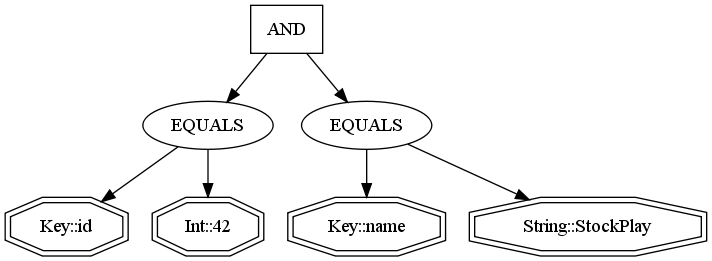
\includegraphics[width=\textwidth]{images/realisatie/AST}
	\caption{Abstract Syntax Tree van een voorbeeldfilter.}
\end{figure}


\section{Verwerking}

Nu de semantiek en conversie van onze filter vastligt, konden we starten met de effectieve implementatie ervan: het omzetten naar of toepassen van de filter op een variabele data-backend. Hierbij zijn de twee grote pistes direct duidelijk: toepassing, of omzetting.

\subsection{Lokale toepassing}

Bij deze opzet wordt de filter lokaal toegepast op een binnengehaalde dataset. Het idee hierbij was om alle records op te halen, en de filter dan lokaal een selectie te laten maken. Die selectie, die voldoet aan de eisen die door de gebruiker zijn opgelegd, kan dan teruggestuurd worden.

Hoewel dit idee perfect toepasbaar is bij systemen waar alle data lokaal aanwezig is (zoals een lokale Java data-backend), treden er problemen op als de data enkel remote aanwezig is en lokaal niet gecachet wordt. In dit geval wordt de overhead van het ophalen van alle records veel te groot, zeker toegepast op StockPlay waarbij de Securities-tabel gemakkelijk meer dan duizend records kan bevatten. Hoewel deze evaluatietechniek dus eenvoudiger te implementeren is (het data-backend-specifieke gedeelte is niet meer aanwezig), hebben we door de grote overhead besloten een alternatief te zoeken.

\subsection{Omzetting}

Het alternatief voor een lokale toepassing, is een omzetting van de filter-boom naar een formaat dat geschikt is om op afstand verwerkt te worden. Hierbij is er geen overhead meer aanwezig, maar wordt het geheel een pak complexer daar het moet kunnen omgezet worden naar een specifieke syntax, afhankelijk van de data-backend.

Om dit te kunnen realiseren, hebben we eerst voorzien in een pseudo-abstracte klasse (Convertable, wel instantieerbaar, maar de compile() functie is ``verboden'') die voorziet in een interface en gemeenschappelijke functionaliteit, onder meer voor het verwerken van eventuele parameters. Filter sub-objecten (Condities, Relaties, en Data objecten) breiden vervolgens deze abstracte klasse gepast uit, door niet zozeer functionaliteit toe te voegen, maar louter voorziet in een hi\"erarchie (zo kunnen we later bijvoorbeeld zeggen dat een Condition enkel Data-objecten als argumenten kan aanvaarden).
Het volgend niveau in het Filter model is dat van de effectieve Condities, Relaties, en Datatypes. Een dergelijke klasse (vb ConditionEquals) breidt opnieuw zijn ouder uit, waarbij de toegevoegde functionaliteit bestaat uit het opbouwen van een graaf-subtree (meer hierover later), het specificeren van een functiesignatuur, en het vereisen van een \emph{compile()} functie voor alle implenterende klassen.
Het finale niveau in ons model voorziet in een implementatie van bovenstaande objecten. Zo zal elke Convertable een implementatie moeten hebben voor elke data-backend (bijvoorbeeld sql.ConditionEquals). Via introspectie zal een Convertable at-runtime een correcte implementatie instantieren, wiens \emph{process()} functie dan instaat voor het genereren van een object dat bruikbaar is voor een data-backend (in geval van SQL zal dit een String).

Deze opzet (pseudo-abstracte Convertable objecten die opnieuw een Convertable instanti\"eren die nu wel over een compile() functie beschikt) mag misschien complex lijken, maar het is elementair in het generiek maken van de filters. Aangezien de pseudo-abstracte Convertable objecten rechtstreeks instantieerbaar zijn, kan de Parser een boomstructuur aan dergelijke objecten opstellen zonder weet te hebben van hoe die boom uiteindelijk zal gecompileerd worden. Het is slechts wanneer die aanroep effectief gebeurt, dat elk Convertable object zal opvragen hoe hij gecompileerd moet worden, om zo de juiste Converter op te roepen. Die Converters voorzien ook niet in een \emph{compile()} instructie, omdat die instructie geen parameters vastlegt en dus manueel de private dataleden zou moeten raadplegen om parameters op te halen. Om dit te vermijden hebben we gekozen voor een extra instructie, de \emph{process()} instructie, die w\'el voorziet in een specifieke signatuur om zo verkeerde implementaties van de Convertables te vermijden.

\begin{code}
\begin{verbatim}
id = 42 AND name = "StockPlay"
\end{verbatim}
\caption{Finaal resultaat na omzetting door de SQL-converters.}
\end{code}


\section{Syntaxreferentie}

Zoals reeds beschreven bestaat een filter essenti\"eel uit drie verschillende mogelijke objecten: condities, relaties, en data-objecten. In deze sectie documenteren we die types, en de exacte grammatica die gebruikt moet worden.

\subsection{Operatoren}

\begin{itemize}
\item{Ronde haakjes: wordt gebruikt om conditities en relaties te groeperen om precedentie in te voeren.}
\item{Komma: wordt gebruikt om de argumenten die aan een functie doorgegeven worden, te scheiden (momenteel ongebruikt).}
\end{itemize}

Ronde haakjes zijn nodig wanneer precedentie onduidelijk is. Aangezien er geen niveaus van precendentie gedefini\"eerd zijn tussen verschillende relaties, zullen er altijd haken moeten gebruikt worden wanneer er zich verschillende relaties in eenzelfde filter bevinden. Bij gelijke relaties wordt er echter impliciet linkse-precedentie toegepast, en zijn haken niet vereist.

\begin{code}
\begin{verbatim}
-- door de impliciete linkse-precedentie wordt eerst de
-- id-expressie ge\"evalueerd, vervolgens de age-expressie en
-- tenslotte de name-expressie.
id >= 5 && age >= 10 && name != 'Jan's

\end{verbatim}
\caption{Demonstratie van de impliciete linkse-precedentie.}
\end{code}

\subsection{Datatypes}

De verschillende datatypes kunnen op verschillende manieren opgesteld worden: rechtstreeks, of indirect. De directe manier is echter enkel beschikbaar voor primitieve dataobjecten (integers, floating-point getallen, strings, en sleutels). Hierbij moet de gebruiker louter de waarde van het getal invoegen in de filter, en zal de parser detecteren om welk formaat het gaat.
Indirecte contructie is steeds mogelijk, en is some de enige optie (bij complexere dataobjecten). Hierbij geeft de gebruiker de data in als een \emph{quoted string} (die voldoet aan een vaste grammatica), en zal een karakter na de laatste quote (de \emph{modifier}) indiceren om welk datatype het gaat.

\subsubsection{Sleutels}

Dit speciaal datatype wordt gebruikt om bij een conditie een specifieke kolom te selecteren. Het mag enkel bestaan uit alfabetische karakters (zowel lower- als uppercase), en een \_ symbool. Het wordt niet omringd door aanhalingstekens, indien dit wel het geval zou zijn wordt het gewoon ge\"interpreteerd als een reguliere string.

\begin{code}
\begin{verbatim}
-- id is een sleutel: verwijst naar een specifieke kolom om de
-- gelijkheids-conditie op in te laten werken
id EQUALS 5
\end{verbatim}
\caption{Illustratief gebruik van een sleutel.}
\end{code}

\subsubsection{Tekenreeksen}

Dit datatype stelt een ordinaire string voor, en kan alle karakters omvatten op voorwaarde dat het omsloten wordt door enkele quotes (en mag er dus geen bevatten, \emph{escaping} wordt niet ondersteund. Zoals wellicht zal opvallen lijkt deze notatie sterk op de indirecte constructiemethode die kan gebruikt worden voor andere datatypes, en eigenlijk is het ook zo geimplementeerd: bij afwezigheid van een modifier na de laatste quote wordt die impliciet verondersteld als zijnde een 's', de modifier voor strings.

\begin{code}
\begin{verbatim}
name EQUALS 'Foo'
name EQUALS 'Foo's
\end{verbatim}
\caption{Illustratief gebruik van een tekenreeks.}
\end{code}

\subsubsection{Natuurlijke getallen -- int}

Dit primitief datatype wordt gebruikt om natuurlijk getallen te detecteren, en mag enkel getallen bevatten (eventueel voorafgegaan door een minteken). Het datatype kan rechtstreeks geconstrueerd worden, en bij indirecte constructie wordt het voorgesteld door de modifier 'i'.

\begin{code}
\begin{verbatim}
id EQUALS 5
id EQUALS '5'i
\end{verbatim}
\caption{Illustratief gebruik van een natuurlijk getal.}
\end{code}

\subsubsection{Gehele getallen -- float}

Dit is een uitbreiding van de natuurlijke getallen, en mag zo ook een decimaal punt bevatten om kommagetallen aan te duiden. Het datatype kan rechtstreeks geconstrueerd worden, en bij indirecte constructie wordt het voorgesteld door de modifier 'f'.

\begin{code}
\begin{verbatim}
cash EQUALS 123.45
cash EQUALS '123.45'f
\end{verbatim}
\caption{Illustratief gebruik van een geheel getal.}
\end{code}

\subsubsection{Datums -- date}

Dit is een voorbeeld van een complex type dat enkel kan geconstrueerd worden via de indirecte methode, gebruik makend van modifier 'd'. Aangezien datums op verschillende manieren kunnen voorgesteld worden, accepteren we enkel volgende methoden (gestandaardiseerd in ISO 8601):
\begin{itemize}
\item{YYYY-MM-DD: 2010-04-07}
\item{YYYY-MM-DD'T'HH:MM'Z': 2010-04-07T05:56Z}
\end{itemize}

Uren zijn steeds in 24-uurs formaat, gespecificeerd in de UTC-tijdzone. Bij afwezigheid van het uur (vb. in YYYY-MM-DD), wordt dit impliciet ingesteld op '00:00' (middernacht), en zal ook zo in de database-backend verwerkt worden. De converters hebben dus geen weet van de manier waarop de datum ingegeven is (al dan niet met gespecificeerd uur).

\begin{code}
\begin{verbatim}
date EQUALS '2010-04-07'd
date EQUALS '2010-04-07T16:01Z'd
\end{verbatim}
\caption{Illustratief gebruik van een datum.}
\end{code}

\subsubsection{Reguliere expressies -- regex}

Dit complex datatype wordt steeds gebruikt in combinatie met de LIKE operator, en kan enkel geconstrueerd worden via de indirecte methode, gebruik makend van de modifier 'r'. Dit datatype ondersteund als enige ook extra modifiers, die het gedrag van de reguliere expressie verfijnen. De volgende extra modifiers worden ondersteund:
\begin{itemize}
\item 'i' modifier: zorgt dat de reguliere expressie case-insensitive werkt
\end{itemize}

\begin{code}
\begin{verbatim}
name LIKE '^j*n$'ri
\end{verbatim}
\caption{Illustratief gebruik van een reguliere expressie.}
\end{code}

\subsection{Condities}

Een conditie wordt gebruikt om een specifieke vergelijkingsoperatie toe te passen op een kolom, zodat er een selectie gebeurd op basis van deze conditie. De mogelije condities (met tussen haken de signatuur) zijn:

\begin{itemize}
\item == of EQUALS: vereist dat twee velden identiek zijn [Key, *]
\item != of NOTEQUALS: vereist dat twee velden verschillend zijn [Key, *]
\item > of GREATHERTHAN: vereist dat het ene veld groter is dan het andere [Key, *]
\item < of LESSTHAN: vereist dat het ene veld kleiner is dan het andere [Key, *]
\item >= of GREATHERTHANOREQUAL: vereist dat het ene veld strikt groter is dan het andere [Key, *]
\item <= of LESSTHANOREQUAL: vereist dat het ene veld strikt kleiner is dan het andere [Key, *]
\item =~ of LIKE: vereist dat het ene veld voldoet aan de string (met wildcards) in het tweede veld [Key, String]
\item !~ of NOTLIKE: vereist dat het ene veld verschilt van de string (met wildcards) in het tweede veld [Key, String]
\end{itemize}

\subsection{Relaties}

Relaties dienen om verschillende condities aan elkaar te schakelen, en het resultaat op een specifieke wijze te interpreteren.

\begin{itemize}
\item \&\& of AND
\item $||$ of OR
\end{itemize}

\subsection{Functies}

Momenteel zijn er nog geen functies gedefini\"eerd in de parser, maar de infrastructuur is er op voorzien. Mits een eenvoudige uitbreiding van de tokenizer kan er zelf gebruik gemaakt worden van functies met een variabel aantal argumenten.




% Invoering
\part{Invoering}
%
% Oracle database
%

\chapter{Databases}


%
% Backend
%

\chapter{Backend}

\todo{builden van branched nightlies, oid}


%
% Scraper
%

\chapter{Scraper}


%
% Interfaces
%

\chapter{Interfaces}


% Documentatie
\part{Documentatie}
\todo{Hier komt auto-gegenereerde data van onze code}

%
% Bijlagen
%

\part{Bijlagen}
\appendix

% XML-RPC
\chapter{XML-RPC specificatie}
%
% Overview
%

\section{Overview}

XML-RPC is a Remote Procedure Calling protocol that works over the Internet.
An XML-RPC message is an HTTP-POST request. The body of the request is in XML. A procedure executes on the server and the value it returns is also formatted in XML.
Procedure parameters can be scalars, numbers, strings, dates, etc.; and can also be complex record and list structures.


%
% Specification
%

\section{Specification}

\subsection{Request example}

Here's an example of an XML-RPC request:
\begin{verbatim}
POST /RPC2 HTTP/1.0
User-Agent: Frontier/5.1.2 (WinNT)
Host: betty.userland.com
Content-Type: text/xml
Content-length: 181

<?xml version="1.0"?>
<methodCall>
  <methodName>examples.getStateName</methodName>
  <params>
    <param>
      <value><i4>41</i4></value>
    </param>
  </params>
</methodCall>
\end{verbatim}

\subsection{Header requirements}

The format of the URI in the first line of the header is not specified. For example, it could be empty, a single slash, if the server is only handling XML-RPC calls. However, if the server is handling a mix of incoming HTTP requests, we allow the URI to help route the request to the code that handles XML-RPC requests. (In the example, the URI is /RPC2, telling the server to route the request to the "RPC2" responder.)

A User-Agent and Host must be specified.

The Content-Type is text/xml.

The Content-Length must be specified and must be correct.

\subsection{Payload format}

The payload is in XML, a single $<$methodCall$>$ structure.

The $<$methodCall$>$ must contain a $<$methodName$>$ sub-item, a string, containing the name of the method to be called. The string may only contain identifier characters, upper and lower-case A-Z, the numeric characters, 0-9, underscore, dot, colon and slash. It's entirely up to the server to decide how to interpret the characters in a methodName.

For example, the methodName could be the name of a file containing a script that executes on an incoming request. It could be the name of a cell in a database table. Or it could be a path to a file contained within a hierarchy of folders and files.

If the procedure call has parameters, the $<$methodCall$>$ must contain a $<$params$>$ sub-item. The $<$params$>$ sub-item can contain any number of $<$param$>$s, each of which has a $<$value$>$.

\subsection{Scalar $<$value$>$s}

$<$value$>$s can be scalars, type is indicated by nesting the value inside one of the tags listed in this table:

\begin{table}
\caption{Possible scalar values}
\centering
\begin{tabular}{ccccccc}
\hline \hline
\textbf{Tag} & \textbf{Type} & \textbf{Example} \\
\hline
$<$i4$>$ or $<$int$>$ & four-byte signed integer & -12 \\
$<$boolean$>$ & 0 (false) or 1 (true) & 1 \\
$<$string$>$ & string & hello world \\
$<$double$>$ & double-precision signed floating point number & -12.214 \\
$<$dateTime.iso8601$>$ & date/time & 19980717T14:08:55 \\
$<$base64$>$ & base64-encoded binary & eW91IGNhbid0IHJlYWQgdGhpcyE= \\
\hline
\end{tabular}
\end{table}

If no type is indicated, the type is string.

\subsection{$<$struct$>$s}

A value can also be of type $<$struct$>$.

A $<$struct$>$ contains $<$member$>$s and each $<$member$>$ contains a $<$name$>$ and a $<$value$>$.

Here's an example of a two-element $<$struct$>$:
\begin{verbatim}
  <struct>
  <member>
    <name>lowerBound</name>
    <value><i4>18</i4></value>
  </member>
  <member>
    <name>upperBound</name>
    <value><i4>139</i4></value>
  </member>
</struct>
\end{verbatim}

$<$struct$>$s can be recursive, any $<$value$>$ may contain a $<$struct$>$ or any other type, including an $<$array$>$, described below.
\subsection{$<$array$>$s}

A value can also be of type $<$array$>$.

An $<$array$>$ contains a single $<$data$>$ element, which can contain any number of $<$value$>$s.

Here's an example of a four-element array:
\begin{verbatim}
<array>
  <data>
    <value><i4>12</i4></value>
    <value><string>Egypt</string></value>
    <value><boolean>0</boolean></value>
    <value><i4>-31</i4></value>
  </data>
</array>
\end{verbatim}

$<$array$>$ elements do not have names.

You can mix types as the example above illustrates.

$<$arrays$>$s can be recursive, any value may contain an $<$array$>$ or any other type, including a $<$struct$>$, described above.
\subsection{Response example}

Here's an example of a response to an XML-RPC request:
\begin{verbatim}
HTTP/1.1 200 OK
Connection: close
Content-Length: 158
Content-Type: text/xml
Date: Fri, 17 Jul 1998 19:55:08 GMT
Server: UserLand Frontier/5.1.2-WinNT

<?xml version="1.0"?>
<methodResponse>
  <params>
    <param>
      <value><string>South Dakota</string></value>
    </param>
  </params>
</methodResponse>
\end{verbatim}
\subsection{Response format}

Unless there's a lower-level error, always return 200 OK.

The Content-Type is text/xml. Content-Length must be present and correct.

The body of the response is a single XML structure, a $<$methodResponse$>$, which can contain a single $<$params$>$ which contains a single $<$param$>$ which contains a single $<$value$>$.

The $<$methodResponse$>$ could also contain a $<$fault$>$ which contains a $<$value$>$ which is a $<$struct$>$ containing two elements, one named $<$faultCode$>$, an $<$int$>$ and one named $<$faultString$>$, a $<$string$>$.

A $<$methodResponse$>$ can not contain both a $<$fault$>$ and a $<$params$>$.
\subsection{Fault example}
\begin{verbatim}
HTTP/1.1 200 OK
Connection: close
Content-Length: 426
Content-Type: text/xml
Date: Fri, 17 Jul 1998 19:55:02 GMT
Server: UserLand Frontier/5.1.2-WinNT

<?xml version="1.0"?>
<methodResponse>
  <fault>
    <value>
    <struct>
      <member>
        <name>faultCode</name>
        <value><int>4</int></value>
      </member>
      <member>
        <name>faultString</name>
        <value><string>Too many parameters.</string></value>
      </member>
    </struct>
    </value>
  </fault>
</methodResponse>
\end{verbatim}


%
% Strategies and goals
%

\section{Strategies and goals}

\emph{Firewalls}: the goal of this protocol is to lay a compatible foundation across different environments, no new power is provided beyond the capabilities of the CGI interface. Firewall software can watch for POSTs whose Content-Type is text/xml.

\emph{Discoverability}: we wanted a clean, extensible format that's very simple. It should be possible for an HTML coder to be able to look at a file containing an XML-RPC procedure call, understand what it's doing, and be able to modify it and have it work on the first or second try.

\emph{Easy to implement}: we also wanted it to be an easy to implement protocol that could quickly be adapted to run in other environments or on other operating systems.


%
% Updates
%

\section{Updates}

\subsection{As of 1/21/99 DW}

The following questions came up on the UserLand discussion group as XML-RPC was being implemented in Python.
\begin{itemize}
\item The Response Format section says "The body of the response is a single XML structure, a $<$methodResponse$>$, which \emph{ can}
contain a single $<$params$>$..." This is confusing. Can we leave out the $<$params$>$? 

No you cannot leave it out if the procedure executed successfully. There are only two options, either a response contains a $<$params$>$ structure or it contains a $<$fault$>$ structure. That's why we used the word "can" in that sentence.

\item Is "boolean" a distinct data type, or can boolean values be interchanged with integers (e.g. zero=false, non-zero=true)? 

Yes, boolean is a distinct data type. Some languages/environments allow for an easy coercion from zero to false and one to true, but if you mean true, send a boolean type with the value true, so your intent can't possibly be misunderstood.

\item What is the legal syntax (and range) for integers? How to deal with leading zeros? Is a leading plus sign allowed? How to deal with whitespace? 

An integer is a 32-bit signed number. You can include a plus or minus at the beginning of a string of numeric characters. Leading zeros are collapsed. Whitespace is not permitted. Just numeric characters preceeded by a plus or minus.

\item What is the legal syntax (and range) for floating point values (doubles)? How is the exponent represented? How to deal with whitespace? Can infinity and "not a number" be represented? 

There is no representation for infinity or negative infinity or "not a number". At this time, only decimal point notation is allowed, a plus or a minus, followed by any number of numeric characters, followed by a period and any number of numeric characters. Whitespace is not allowed. The range of allowable values is implementation-dependent, is not specified.

\item What characters are allowed in strings? Non-printable characters? Null characters? Can a "string" be used to hold an arbitrary chunk of binary data? 

Any characters are allowed in a string except $<$ and \&, which are encoded as \&lt; and \&amp;. A string can be used to encode binary data.

\item Does the "struct" element keep the order of keys. Or in other words, is the struct "foo=1, bar=2" equivalent to "bar=2, foo=1" or not? 

The struct element does not preserve the order of the keys. The two structs are equivalent.

\item Can the $<$fault$>$ struct contain other members than $<$faultCode$>$ and $<$faultString$>$? Is there a global list of faultCodes? (so they can be mapped to distinct exceptions for languages like Python and Java)? 

A $<$fault$>$ struct \textbf{may not}
contain members other than those specified. This is true for all other structures. We believe the specification is flexible enough so that all reasonable data-transfer needs can be accomodated within the specified structures. If you believe strongly that this is not true, please post a message on the discussion group.

There is no global list of fault codes. It is up to the server implementer, or higher-level standards to specify fault codes.

\item What timezone should be assumed for the dateTime.iso8601 type? UTC? localtime? 

Don't assume a timezone. It should be specified by the server in its documentation what assumptions it makes about timezones.
\end{itemize}

There have been additions as well:
\begin{itemize}
\item $<$base64$>$ type. 1/21/99 DW.
\end{itemize}

\subsection{As of 6/30/03 DW}

Removed "ASCII" from definition of string.

Changed copyright dates, below, to 1999-2003 from 1998-99.


%
% Copyright and disclaimer
%

\section{Copyright and disclaimer}

{\copyright} Copyright 1998-2003 UserLand Software. All Rights Reserved.

This document and translations of it may be copied and furnished to others, and derivative works that comment on or otherwise explain it or assist in its implementation may be prepared, copied, published and distributed, in whole or in part, without restriction of any kind, provided that the above copyright notice and these paragraphs are included on all such copies and derivative works.

This document may not be modified in any way, such as by removing the copyright notice or references to UserLand or other organizations. Further, while these copyright restrictions apply to the written XML-RPC specification, no claim of ownership is made by UserLand to the protocol it describes. Any party may, for commercial or non-commercial purposes, implement this protocol without royalty or license fee to UserLand. The limited permissions granted herein are perpetual and will not be revoked by UserLand or its successors or assigns.

This document and the information contained herein is provided on an "AS IS" basis and USERLAND DISCLAIMS ALL WARRANTIES, EXPRESS OR IMPLIED, INCLUDING BUT NOT LIMITED TO ANY WARRANTY THAT THE USE OF THE INFORMATION HEREIN WILL NOT INFRINGE ANY RIGHTS OR ANY IMPLIED WARRANTIES OF MERCHANTABILITY OR FITNESS FOR A PARTICULAR PURPOSE.

\end{document}



% Woordenboek
\chapter{Woordenboek}
%
% Configuratie
%

% Label
\label{chap:woordenboek}


%
% Financiële terminologie
%

\section{Financi\"ele terminologie}


%
% Technische terminologie
%

\section{Technische terminologie}



\printindex
\end{document}

